\documentclass{article}
\usepackage[round]{natbib}
\usepackage{amsmath,amssymb,amsfonts}%
\usepackage{geometry}%
\usepackage{color}
\usepackage{graphicx}
\usepackage{authblk}
\usepackage{nameref}
\usepackage[right]{lineno}
\usepackage{subcaption}
\usepackage{tikz}
\usetikzlibrary{calc,positioning}
\usepackage{url}
% JK: turning this off for the moment as I keep clicking through on links
% to the bibliography while reading the text and it's intensely annoying.
% Can reinstate when we're ready to preprint
% \usepackage[hidelinks]{hyperref}

\newcommand{\noderef}[1]{\textsf{#1}}
\newcommand{\tsinfer}[0]{\texttt{tsinfer}}
\newcommand{\kwarg}[0]{\texttt{KwARG}}
\newcommand{\argweaver}[0]{\texttt{ARGweaver}}
\newcommand{\relate}[0]{\texttt{Relate}}
\newcommand{\espalier}[0]{\texttt{Espalier}}

\begin{document}

\linenumbers
\title{A general and efficient representation of Ancestral Recombination Graphs}

% First authors
\author[1]{Yan Wong}

% Second authors
\author[2,$\star$]{Anastasia Ignatieva}
\author[3,$\star$]{Jere Koskela}

% Middle Authors
\author[4]{Gregor Gorjanc}
\author[5]{Anthony W. Wohns}

% Corresponding
\author[1,$\dagger$]{Jerome Kelleher}

\affil[1]{Big Data Institute, Li Ka Shing Centre for Health Information and Discovery, University of Oxford, OX3 7LF, UK}
\affil[2]{Department of Statistics, University of Oxford, OX1 3LB, UK}
\affil[3]{Department of Statistics, University of Warwick, CV4 7AL, UK}
\affil[4]{The Roslin Institute and Royal (Dick) School of Veterinary Studies, University of Edinburgh, EH25 9RG, UK}
\affil[5]{Broad Institute of MIT and Harvard, Cambridge, MA 02142, USA}

\affil[$\star$]{Denotes shared second authorship, listed alphabetically}
\affil[$\dagger$]{Denotes corresponding author}


\maketitle

% JK: this is a rough first pass for a slightly different paper. Needs
% substantial revision.
\begin{abstract}
It has recently become possible to infer genetic ancestry in the presence of
recombination at scale for the first time, enabling many
downstream applications in population and statistical genetics.
Such recombinant genetic ancestry is usually
referred to as an Ancestral Recombination Graph, or ARG.
% Note: slight repetition here with first sentence.
There are now multiple methods that can infer ARGs at a practical scale
and it is therefore vital that these methods can be systematically evaluated
and compared to determine their strengths and weaknesses.
Unfortunately confusion exists over terminology and there is
little agreement on shared standards for data interchange,
significantly hampering progress in the field.
This lack of clarity and agreement on basic issues such as what does and
does not constitute an ARG is partly attributable to the historical
development of the term.
Originally rigorously defined as
a stochastic process (the coalescent with recombination) together with its
representation, an ARG is now understood to refer to any
concrete realisation of a recombinant genetic ancestry.
We show that the standard description of an ARG
in terms of common ancestor and recombination events
(inherited from the original stochastic process definition) is
ambiguous,
% is it ambiguous? How? Can we simply delete this?
fundamentally limited and an unsuitable basis for data interchange.
We provide a simple alternative definition of an ARG in which a node
corresponds to one of an individual's monoploid genomes and an edge
defines genetic inheritance between two nodes, with annotations on
each edge specifying which regions of the genome have
been inherited via that route.
We show how this definition can be used to generalise the encoding to
cover both the standard and several simplified versions of ARGs, as well as
enabling efficient access to local trees along the genome. Additionally, we
define some classifications and metrics of ARG nodes. Finally, we relate
these generalisations to the ARGs produced by a number of recently
developed ancestral inference methods.
% jk-note: this ends a bit flat - we should say other stuff like we clarify
% how the ARG relates the pedigree, etc, etc. Let's go through again when
% we have a reasonable draft.
\end{abstract}

\textbf{Keywords:} Ancestral Recombination Graphs

\section*{Introduction}
Inferring the genetic relationships between sampled genomes in the form of an
evolutionary or phylogenetic tree is a necessary prerequisite for many analyses of
species~\citep{rannala2003genetics}, non-recombining sections of
DNA~\citep{cann1987mitochondrial,underhill2001annalsofhumangenetics}
and viruses~\citep{grenfell2004science}.
A phylogenetic tree captures information about the genealogy
of the sample in an elegant and concise
way, by postulating a set of ancestors common to the samples
together with paths of inheritance between them. A rich literature exists
on analysing the mathematical properties of these
trees~\citep{steel2016phylogeny}, and numerous
methods exist to infer them~\citep{felsenstein2004inferring}.
However, the genetic genealogy of a recombining organism
cannot be described as a single evolutionary tree: instead,
the inheritance of each local section of the genome may be described
by a (slightly) different tree~\citet{hudson1983properties}. Inferring complex
genealogies of this nature
presents profound technical difficulties, meaning tree-based approaches are
rarely used in population and statistical genetics. Therefore until recently, analysis of
population genetic data has primarily focussed on summaries derived
from the local trees~\citep{tajima1983evolutionary,tavare1984line}
rather than using the underlying genealogy itself. Such
derived measures include allele frequencies and site frequency
spectra~\citep{achaz2009frequency,ralph2020efficiently},
patterns of linkage disequilibrium~\citep{mcvean2002genealogical}, and
principal components~\citep{mcvean2009genealogical}.

Recent breakthroughs in large-scale inference
methods~\citep{rasmussen2014genome,kelleher2019inferring,speidel2019method,wohns2022unified}
and data representation~\citep{kelleher2016efficient}
have raised the realistic prospect of genealogical analysis becoming a standard part
of the population and statistical genetics toolkit~\citep{hejase2020summary}.
Applications using these inferred ancestries as input have begun to
appear~\citep{osmond2021estimating,zhang2021biobank,fan2022genealogical,hejase2022deep}
and many more are sure to
follow~\citep{harris2019database}. This vibrant research area, however,
has a significant difficulty, which risks hampering
progress: we currently lack a well-defined data-model and shared terminology
to discuss recombining genealogies. This leads to basic errors in statements
about what different inference methods produce as output, as well as presenting serious
difficulties in either comparing the outputs of different methods or
(from a user's perspective) using multiple inference methods in an analysis.

In this paper we [turn into proper round up paragraph later]
\begin{enumerate}
\item Discuss the classical Ancestral Recombination Graph formulation,
and show how it derives from (and is limited by) the coalescent with
recombination.
\item Suggest a definition of ARGs that is free of these limitations,
where the formulation is derived from a (normally diploid) pedigree rather than from
coalescent approximations, and where the genetic
material which is transmitted is described by annotations attached to
edges rather than nodes.
\item Suggest a classification of ARG nodes that helps us to understand
the properties of the structures inferred by different methods, and illustrate
with some examples.
% Perhaps we should also mention something about simplification and unknowable
% nodes, e.g. ``show how some of the nodes are not required for useful interpretation
% of ancestry''.
\item Despite its status as ``the ideal data structure for
population genomic analysis''~\citep{rasmussen2014genome}, there has been
little discussion of its computational properties. We discuss the
relationship between the classical concept of an ARG and the
recently introduced succinct tree sequence data structure.
\end{enumerate}

\section*{Ancestral graphs: a brief history}
The coalescent~\citep{kingman1982coalescent,kingman1982genealogy,
hudson1983testing, tajima1983evolutionary} models the ancestry of a sample of
genomes under an idealised population model, and provides the theoretical
underpinning for much of contemporary population genetics.
It is a stochastic process, where each random realisation
is a genealogical tree describing the genetic ancestry of the samples.
Numerous elaborations have been incorporated into the
basic process~\citep{hudson1990gene,hein2004gene,wakely2008coalescent};
in particular, early work by \citet{hudson1983properties}
analysed the effects of recombination on the random genealogical
trees generated by the coalescent. This
generated several fundamental analytical results
as well as describing the elegant algorithm
at the heart of simulation
programs~\citep{hudson2002generating,kelleher2016efficient,baumdicker2021efficient}
used in thousands of studies.
In its original formulation, Hudson's algorithm produced a
sequence of genealogical trees along the genome.
Critically, although the correlation structure among these
local trees was analysed analytically, those correlations
were not captured explicitly: the ancestry
was viewed as a series of disconnected local trees rather than
as a single cohesive object.

In the 1990s, Griffiths and colleagues revisited the
coalescent with recombination from a different perspective,
in which the stochastic process itself is encoded as a graph,
and showed how the local trees generated by Hudson's algorithm
were embedded within
it~\citep{griffiths1991two,ethier1990two,griffiths1996ancestral,griffiths1997ancestral}.
They referred to this graph,
representing both the stochastic process and
its random realisations, as the Ancestral Recombination Graph (ARG).
Although mathematically equivalent, it is
important to note that the Griffiths and Hudson formulations of
the coalescent with recombination are not identical;
in particular, a direct implementation of the ARG process
requires exponential time to simulate
(see Appendix XXX for details). However, ARGs provided a way
to describe recombinant ancestry as single object that
could be reasoned about and inferred in a way
that was missing from Hudson's treatments.

Early work on ARG inference focused on the problem of
inferring parameters of the
stochastic process, where the ancestry was regarded as a
latent parameter to be averaged out
\citep[e.g.][]{griffiths1996ancestral,kuhner2000maximum, nielsen2000estimation,
fearnhead2001estimating}.
These methods met with limited success
because the state space of ARGs is overwhelmingly large and
lacks a simple geometry or neighbourhood structure for inference or
sampling methods to  exploit.
The focus subsequently shifted to the more
tractable---but still NP-hard~\citep{wang2001perfect}---problem of computing
the minimum number of recombinations required
to explain an input dataset~\citep{myers2003bounds}, and inferring the corresponding
ARG realisations~\citep{song2003parsimonious,song2005efficient,lyngso2005minimum}.
It is important to note that such recombination-parsimony ARGs
have quite different properties from realisations of the
ARG \emph{process} as modelled by Hudson, Griffiths, and colleagues.
Firstly, branch lengths are not typically estimated,
% why do we need the following two lines
and node times are required in order to compute a likelihood under the
coalescent with recombination (see section XXX).
Secondly, even if branch lengths were estimated,
the realisations would have a very small likelihood since
the coalescent with recombination is often highly \emph{un}parsimonious
in terms of recombination events.
The previously close correspondance
between the ARG as a mathematical representation of the coalescent process
and as concrete realisations of ancestry was therefore broken.
\cite{minichiello2006mapping} explicitly distinguished the ARG as a
stochastic process from the ARG as a data structure, and
argued for using the term to mean specific realised ancestral histories.
This has become a common
usage~\citep[e.g.][]{gusfield2014recombinatorics,mathieson2020ancestry,brandt2021evaluation},
although not universal, with authors also using the term
in the original stochastic
process sense~\citep[e.g.][]{nordborg2000linkage,birkner2013ancestral,
wilton2015smc,griffiths2016coalescent}.

% Gusfield~\citep{gusfield2014recombinatorics}
% defines also defines an ARG as a concrete realisation
% and studies instances that satisfy particular
% properties such as ``galled trees''
% \citep{wang2001perfect, gusfield2004optimal}
% as well as describing algorithms for more general phylogenetic
% networks~\citep{huson2010phylogenetic}.

% JK: This paragraph is weak, and needs some work. Basically want to
% illustrate the mathematical literature which views ancestral
% graphs very much as *processes*.
% Jere: ASG section redrafted, gene transfer left as TODO (because I
% know essentially nothing about it).
In parallel with this tendency to decouple the term
Ancestral Recombination Graph from the stochastic process,
an extensive mathematical literature has developed in
studying other related stochastic processes encoded via a graph.
In particular, the Ancestral Selection Graph
(ASG)~\citep{krone1997ancestral,neuhauser1997genealogy}
uses a similar approach to model natural selection.
Unlike the ARG process, the ASG imposes a hard distinction between the stochastic process,
which constructs a random ARG-like graph, and an observable realisation,
which is a single tree sampled from the graph in a non-uniform way to encode desired
patterns of natural selection.
Constructions of ASG-like stochastic processes encoding various
forms of selection, often in parallel with recombination or other genetic forces,
are an area of considerable and ongoing theoretical interest~\citep[e.g.][]{
neuhauser1999ancestral,
donnelly1999genealogical,
fearnhead2001perfect,
fearnhead2003ancestral,
etheridge2009coalescent,
gonzalezcasanova2018duality,
koskela2019robust}.

The point of this historical overview is to illustrate that the term
Ancestral Recombination Graph has different meanings in different
contexts, and in its original form it was closely coupled to
the coalescent with recombination. In the following sections we
show that, although the ARG-as-a-data-structure perspective is
now the most common interpretation, the \emph{form} of that
data structure is still closely linked to the original
stochastic process, and that this form is inflexible
in the types of genetic inheritance that can be described,
computationally inefficient, and
forces complete (and potentially spurious) precision about
the location and timing
of recombination events. % (and coalescent events?)
Unless otherwise stated, we will use the ARG-as-a-data-structure
interpretation for the remainder of this paper.

\section*{Event ARGs}\label{eARG}
In keeping with its original derivation in terms of a stochastic
process, the classical definition of an ARG data structure is
in terms of \emph{events}. Nodes represent
common ancestor or recombination events that occurred in the
history of some set of sample genomes, and edges represent ancestral
lineages~\citep{griffiths1996ancestral}.
In order to distinguish this form of ARG from what we will be discussing
in later sections we refer to it as an ``event ARG``, or eARG for brevity.
An example of this form of an eARG
is given in Fig.~\ref{fig-arg-data-structure}B.
In a common ancestor event the inbound lineages are merged into a
single ancestral lineage (e.g., node \noderef{e}
in Fig.~\ref{fig-arg-data-structure}), and in a recombination
event a lineage is split into two independent
ancestral lineages (e.g., node \noderef{d}
in Fig.~\ref{fig-arg-data-structure}). The final vital
detail---which distinguishes an arbitrary graph with the required topological
properties from an ARG---is that we associate a breakpoint with each recombination
event. This information is sufficient to uniquely
define the local genealogical trees at every position along the genome,
which is the basic requirement for a data structure encoding
genome-wide genetic ancestry.

\begin{figure}
\centering
% \begin{tabular}{cc}
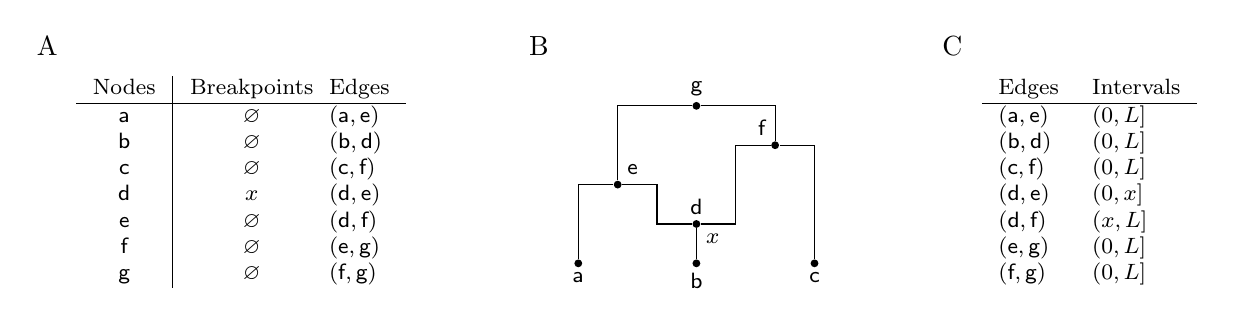
\begin{tikzpicture}[x=5mm, y=5mm, node distance=2mm and 20mm]
\tikzset{greynode/.style={circle,fill,inner sep=1},
nodelabel/.style={font=\footnotesize}}

\node (s0) [greynode] at (0, 0) {};
\node (s1) [greynode] at (3, 0) {};
\node (s2) [greynode] at (6, 0) {};
\node (s3) [greynode] at (3, 1) {};
\node (s4) [greynode] at (1, 2) {};
\node (s5) [greynode] at (5, 3) {};
\node (s6) [greynode] at (3, 4) {};

\node [anchor=north west] at (-1.5,6) {B};
\node [nodelabel,anchor=north west] at ($(s3) + (0,0)$) {$x$};
\foreach \u/\lab in {s0/$\textsf{a}$, s1/$\textsf{b}$, s2/$\textsf{c}$} \node[nodelabel,anchor=north] at (\u) {\lab};
\foreach \u/\lab in {s4/$\textsf{e}$} \node[nodelabel,anchor=south west] at (\u) {\lab};
\foreach \u/\lab in {s5/$\textsf{f}$} \node[nodelabel,anchor=south east] at (\u) {\lab};
\foreach \u/\lab in {s3/$\textsf{d}$, s6/$\textsf{g}$} \node[nodelabel,anchor=south] at (\u) {\lab};

%% Edges
\draw (s1) -- (s3);
\draw (s0) |- (s4);
\draw (s4) -- (2,2) |- (s3);
\draw (s4) |- (s6);
\draw (s3) -- (4,1) |- (s5);
\draw (s2) |- (s5);
\draw (s5) |- (s6);

\node [anchor=north west] at (-14,6) {A};
\node [nodelabel,anchor=north west] at ($(-13,5)$) {
\begin{tabular}{c|c}
% \multicolumn{2}{c}{Breakpoints}\\
Nodes & Breakpoints\\
\hline
$\textsf{a}$ & $\varnothing$ \\
$\textsf{b}$ & $\varnothing$ \\
$\textsf{c}$ & $\varnothing$ \\
$\textsf{d}$ & $x$ \\
$\textsf{e}$ & $\varnothing$ \\
$\textsf{f}$ & $\varnothing$ \\
$\textsf{g}$ & $\varnothing$ \\
\end{tabular}};

\node [nodelabel,anchor=north west] at ($(-7,5)$) {
\begin{tabular}{l}
Edges\\
\hline
$(\textsf{a}, \textsf{e})$ \\
$(\textsf{b}, \textsf{d})$ \\
$(\textsf{c}, \textsf{f})$ \\
$(\textsf{d}, \textsf{e})$ \\
$(\textsf{d}, \textsf{f})$ \\
$(\textsf{e}, \textsf{g})$ \\
$(\textsf{f}, \textsf{g})$ \\
\end{tabular}};


\node [anchor=north west] at (9,6) {C};
\node [nodelabel,anchor=north west] at ($(10,5)$) {
\begin{tabular}{ll}
Edges & Intervals\\
\hline
$(\textsf{a}, \textsf{e})$ & $(0, L]$ \\
$(\textsf{b}, \textsf{d})$ & $(0, L]$ \\
$(\textsf{c}, \textsf{f})$ & $(0, L]$ \\
$(\textsf{d}, \textsf{e})$ & $(0, x]$ \\
$(\textsf{d}, \textsf{f})$ & $(x, L]$ \\
$(\textsf{e}, \textsf{g})$ & $(0, L]$ \\
$(\textsf{f}, \textsf{g})$ & $(0, L]$ \\
\end{tabular}};


\end{tikzpicture}
\caption{\label{fig-arg-data-structure}
A classical ARG (subfigure B), contrasting node with edge breakpoint annotations.
(A) recombination breakpoint information encoded on \emph{nodes}.
This encoding is limited in the patterns of inheritance that can be
described and requires that edges be ordered to avoid ambiguity.
(C) breakpoint annotations associated with \emph{edges}.
Associating the interval of genome inherited by the child node
from the parent with the corresponding edge allows
any pattern genetic inheritance to be described and does
not require edges to be ordered. In this example, each edge is associated
with a single interval, but more generally, multiple non-overlapping intervals
can be associated with a single edge.
}
\end{figure}

% What do we mean by an eARG, formally?
To be concrete, we can formally define the
classical Griffiths eARG as a tuple $(e, \sigma)$, where $e$
is an ordered list of edges defining a directed acyclic graph and
$\sigma: \mathbb{N} \rightarrow \mathbb{N}$
is a function mapping nodes to recombination breakpoints,
such that $\sigma(u) = x$
if $u$ is a recombination event with breakpoint $x$ and
$\sigma(u) = \varnothing$ otherwise.
(This formulation is equivalent to having different ``types''
of node, with breakpoints are associated with recombination
nodes only).
Each edge $e_j = (c, p)$ describes an edge between
child node $c$ and parent $p$, where $c, p \in \mathbb{N}$.
For each recombination node $u$ we must
have exactly two edges in $e$ such that $u$ is the child.
This encoding of an eARG is equivalent to the output
produced by programs such as
\texttt{ARGweaver}~\citep{rasmussen2014genome}
and \texttt{KwARG}~\citep{ignatieva2021kwarg}:
an example is given in Fig.~\ref{fig-arg-data-structure}A.
Note that the description above captures only the
graph topology: if we also wish to know the branch lengths we need
an additional function $t(u): \mathbb{N} \rightarrow \mathbb{R}$
which defines the time of each node.

The ordering of edges is a vital element of the eARG encoding.
This is because there is a fundamental ambiguity involved
in associating recombination breakpoints with nodes
rather than edges: we need to know from which parent the
and the only way we can break this symmetry is to assign
some meaning to the order in which the parents are listed
(\cite{griffiths1997ancestral} refer to the ``left'' and ``right''
parents of a recombination event). This is usually described
in terms of the process in which we extract the local trees
along the genome from an eARG (the most basic downstream
operation for an ARG data structure).
To recover the tree at genome coordinate $x$,
we traverse the graph rootwards from the leaves.
At a particular
node $u$, if it has one parent we are at a common ancestor
node and we follow that parent. If we are at a
recombination node, $u$ has two parents: if
$x$ is less than the breakpoint $\sigma(u)$ we follow
the edge to the first parent, and otherwise follow the edge
to the second parent.
This ordering requirement, while straightforward
to describe, has some practical drawbacks. For example,
% Surely the meaning is clear from the context here and we don't need
% qualify the meaning of ``ARG''
when using this representation and simulating an ARG backwards in time,
the first event above a recombination may involve the lineage carrying the
ancestry to the right of the breakpoint rather
than the left, and so we cannot emit edges as they are generated.
Such issues can be worked around, of course, but depending on the ordering of
otherwise indistinguishable objects is generally problematic. In practice,
several methods explicitly associate information with the outbound edges
of a recombination event
to resolve the issue~\citep{lyngso2005minimum,ignatieva2021kwarg}.

% TODO update this when later sections have been drafted.
As we see in sections XXX and YYY there are substantial limitations
of expressivity and computational performance when using this eARG
encoding. More fundamentally, however, the general approach
of classifying nodes according to a discrete set of events
and associating genome information with those nodes is intrinsically
limiting. As we saw in the previous section, the original ARG
definitions were derived directly from the coalescent with recombination
stochastic process, and the types of ancestry that can be
described are therefore limited by the assumptions of that
model. While the coalescent as a model can be suprisingly robust to
basic violations of the underlying assumptions~\citep{
wakeley2012gene,bhaskar2014distortion,nelson2020accounting},
it is not acceptable that our ability to \emph{represent}
ancestral relationships should be limited by these assumptions.

% n << Ne is a silly assumption in today's datasets
A core assumption of the coalescent is that the sample size $n$
is much less than the effective population size, $N_e$. This
assumption ensures that multiple events (i.e., simultaneous
coalescence and recombination) don't occur at the same
time, which is reflected in the eARG definitions.
This once-reasonable assumption has been overtaken by
the data we have available.
% This can be tightened up a bit, I think. We may need to drop a
% few references.
Several human datasets now consist of hundreds of thousands of
genomes~\citep{bycroft2018genome,karczewski2020mutational,tanjo2021practical},
and so sample size is substantially \emph{larger} than $N_e$
(often assumed to be $10^4$ in humans).
Agricultural datasets are even more extreme.
For example,
the US dairy cattle database alone currently comprises more than 6 million
animals with SNP array
genotypes\footnote{\url{https://queries.uscdcb.com/Genotype/counts.html}},
while the effective population size in modern dairy cattle breeds is
less than 100 and decreasing~\citep{MacLeod2013,Makanjuola2020}.
An extreme sign of these breeding practices is that there are only two ancestral
Y-chromosome linages present in today's US Holstein dairy breed~\citep{Yue2015}.
Simlarly, the 1000 bull genomes project~\citep{hayes20191000}
comprises close to 7000 genomes, which are part of multi-generation pedigrees
with millions of animals and extensive SNP array genotype and phenotype
data \citep[e.g.][]{Cesarani2022}.
Such datasets are also available for other species,
for example, \citet{RosFreixedes2022} have combined genome
and SNP array data to infer recombination of genomes for 440,610 pigs within
7 multi-generation pedigrees~\citep{whalen2018,Johnsson2021,Ros-Freixedes2020}.
Effective population size in modern pig breeds is also less than 100 due to
intense selection and directed reproduction \citep{Hall2016,Porcnic2016}.

Another assumption of the coalescent with recombination which prevents complex
combinations of events occurring simultaneously, is that the genome (or
at least the region under study) is short enough that the number of extant
lineages remains much smaller than $N_e$ at all times. Whole
genome sequences have been available for model organisms
for over a decade now, % True? Citation?
and indeed complete chromosome-level assemblies are possible
in humans~\citep{miga2020telomere}.
Projects are under way to obtain high-quality assemblies
for all eukaryotic species in Britain and Ireland~\citep{darwin2022sequence}
and ultimately worldwide~\citep{lewin2022earth}.
Clearly multiple recombinations (and other complex events) will
occur in the ancestry of such datasets, and we should not be
limited in what we can infer by the data structure that we
use to represent the results.

The eARG encoding consists of two types of event
(common ancestor and recombination) but nature is not so parsimonious
and there are many other processes that will affect the
ancestry of samples.
For example, gene conversion between homologous
chromosomes~\citep{wiuf2000coalescent,chen2007gene} is an important
evolutionary force in many species~\cite[e.g.][]{yang2012great}.
% Some refs for where people are inferring ancestry in the
% presence of GC? Isn't this what ClonalFrame etc are all about?
Similarly, the eARG encoding cannot easily represent multiple
recombinations on a chromosome, or the transmission of multiple
chromosomes.
What we can infer about ancestral histories and
processes should not be limited by the data structure that we
use to represent such ancestry. The eARG is simply one way
to \emph{encode} such history, and, as we have shown,
one that has significant limitations of expressivity
derived from its historical origins in the idealised
coalescent with recombination model.

\section*{Node vs edge annotations}
Another aspect of the classical description of an ARG data structure that
derives from its historical origins as a stochastic
process is how we encode information about genetic
inheritance in the graph. The approach taken by Griffiths to
doing this is concise, elegant: all we need to do is store
the location of the breakpoint at each recombination event.
Storing a breakpoint for each recombinatin event is a very
natural and straightforward thing to do when simulating
a (``Big''; see Appendix XXX) ARG process.
Given the graph topology and these breakpoints, we can then
recover the
local trees at every point in the genome
by tracing rootwards from the leaves and choosing the
appropiate outbound path at recombination nodes.
However, there are several significant disadvantages
to this approach: [TODO be concrete here later
and give pointers to the section where we discuss the
alternative.]

Fortunately, there is a straightforward change to the
classical eARG encoding that simplifies
implementations and greatly increases the flexibility
of both the types and granularity of inheritance information
that we can represent.
The main change that we need to make is to
associate the
the details of inheritance with \emph{edges} rather than
as breakpoints associated with recombination events and
edge ordering rules.
This is illustrated in Fig~\ref{fig-arg-data-structure}C
where this alternative edge annotation formulation is
shown. By associating the interval $(0, x)$ with edge $(d,e)$
and the interval $(x, L)$ with $(d, f)$ we make the encoding
unambiguous: we can list the edges in any order, and it
will describe the same set of local genealogical trees.
This approach is also more flexible, because any pattern
of inheritance can be described by these intervals. For
example, if a gene conversion event occurred where a segment
between positions $x$ and $y$ was inherited by
node $d$ from $e$, we would state this by associating
the intervals $\{(0, x], (y, L]\}$ with $(d,e)$ and
$\{(x, y]\}$ with $(d,f)$.
This change is straightforward, involves no loss of information
and (as we see in later sections)
greatly increases both the expressivity and computational
power of ancestral recombination graph data structures.

\section*{Genome ARGs}
As we have seen in previous sections, the focus
on a limited palette of events makes describing currently-available
datasets and known patterns of genetic inheritance as an eARG
quite cumbersome.
There is no fundamental reason that the patterns of genetic inheritance
that we wish to describe via an ARG must be in terms
of discrete \emph{events}, however. Recent discussions have illustrated the
relationship between ARGs and
the pedigree~\citep{mathieson2020ancestry,brandt2021evaluation},
and the deep connections between the structures are
well understood
\citep[e.g.][]{wakeley2012genetics,gusfield2014recombinatorics,
speed2015naturereviewsgenetics}.
Following \cite{mathieson2020ancestry},
rather defining the inheritance
of genetic material in terms of \emph{events} as we do in an eARG,
we can instead define an ARG data structure in terms of
\emph{genomes} and intervals of genetic inheritance
along the edges (see the previous section).
To distinguish from the classical Griffiths eARG,
we refer to this encoding of an ARG data structure
as a ``Genome ARG'', or gARG.
The distinction between nodes representing events
and genomes may seem pedantic at first, but as we
see in later sections, we gain a great deal of flexibility
and computational efficiency by decoupling our representation
of genetic ancestry from the events that generated it.

\begin{figure}
\begin{center}
    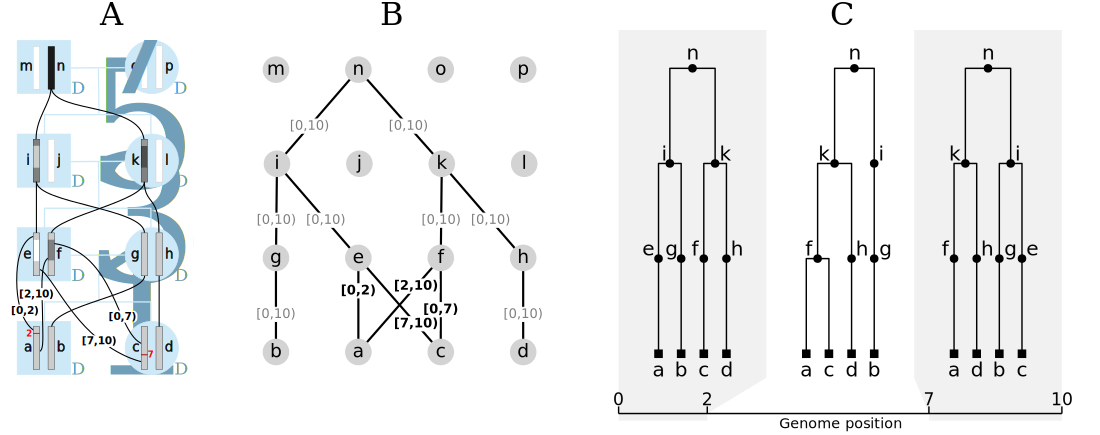
\includegraphics[width=\textwidth]{illustrations/arg-in-pedigree}
\end{center}
\caption{\label{fig-arg-in-pedigree}
% TODO caption needs another pass. One the full section has been written
% it'll be clearer what we need to say in the caption vs the text.
An Ancestral Recombination Graph defined in terms of genomes embedded
in a pedigree. (A) Diploid individuals, visualised in a highly inbred pedigree and
labelled $I_1$ to $I_8$, contain both paternal (left) and maternal (right) genomes
labelled \textsf{a} to \textsf{p}. Black lines show transmission paths connecting
genomes in the current generation (\textsf{a} to \textsf{d}) with their ancestors.
Two recombination breakpoints, at positions 2 and 7 mean that genomes \textsf{a}
and \textsf{c} are independent recombinants of the paternal genomes \textsf{e}
% Gregor: there is some overlap between a and c still (the middle region inherited
% from f) so, a and c are not fully independent!
and \textsf{f}: in these cases the edge annotations have been shown, indicating the
region of genome transmitted. Genomes are shaded such that where, backwards in time,
they merge into a common ancestor, the merged region is darker; this shows that all
genomic regions find a common ancestor in genome \textsf{n} in the oldest generation.
(B) The corresponding genome ARG, where there is a single type of node (representing
a genome) along with annotations on all edges; annotations showing partial
transmission are highlighted in bold. Recombination (e.g.,
the cause of the breakpoint at position 7)
is associated with two parent genomes (\textsf{e} and
\textsf{f}) and a child genome (the recombinant, \textsf{c}).
(C) The edge-annotated genome ARG in (B) fully defines the
local relationships along the genome, as shown in the local
(``marginal'') trees.
}
\end{figure}

A gARG is a graph in which nodes represent monoploid genomes (i.e.,
haploids have one genome, diploids two, etc.) and edges represent
genetic inheritance between an ancestor and a descendant.
Each edge is annotated (see the previous section) with the coordinates
of the genomic intervals over which genetic inheritance occurs
(the next section explores the subtleties of what we mean by
genetic inheritance).
Fig~\ref{fig-arg-in-pedigree} illustrates the basic elements of a gARG,
showing how the genomes embedded in an example (highly inbred)
pedigree correspond to the nodes in a gARG, along with the corresponding
local trees.
A diploid pedigree is shown here for concreteness, but
there is no limitation on mating system, ploidy, or age structure
in the gARG encoding.
In the diploid setting, a genome is inherited from one
of the individual's parents,
and may be the recombined product of that parent's two genomes.
For example, individual $I_1$ in Fig.~\ref{fig-arg-in-pedigree}
has two genomes \textsf{a} and \textsf{b},
inherited from parents $I_3$ and $I_4$. Genome \textsf{a} is the product of
recombining $I_3$'s two genomes \textsf{e} and \textsf{f} at position 2,
whereas \textsf{b} was inherited directly from $I_4$'s genome \textsf{g} without
recombination.
Arbitrary patterns of genetic inheritance (gene conversions, multiple recombinations,
etc) can be expressed without difficulty.

Formally, we can define a gARG as a set of edges $E$, where each
element of the set is a tuple $(c, p, I)$ such that $c, p \in \mathbb{N}$,
$c$ is the child node, $p$ is the parent node and $I$ is the set of
disjoint genomic intervals $(\ell, r]$ over which genome $c$ inherits from $p$ (we may
also phrase this in terms of the ancestral material of a sample---see
the next section).
Deriving the local tree at a point $x$
follows largely the same pattern as for an eARG but is somewhat
simpler because coordinate information is directly associated with
edges. Starting with the sample nodes $S$ we traverse
rootwards through the graph from child to parent. At each node $u$, we find an
edge $(c, p, I) \in E$ such that $u = c$ and $x \in I$
and move to the next node $p$.

There are some interesting and important consequences to this focus on genomes
rather than events.
Firstly, a gARG may contain nodes that are both samples \emph{and}
internal nodes in the local trees.
This ability is useful when we have pedigree information
along with genetic data
\cite[e.g.][]{hayes20191000,RosFreixedes2022,anderson2022genes},
where we may have many generations of internal sample nodes
whose genomes have been sequenced.
Another situation in which it is important that
we do not assume samples are all contemporary ``leaf'' nodes
(or that all internal nodes are either coalescences or recombinations)
is when we are incorporating ancient genomes into ARG
inference~\citep{speidel2021inferring,wohns2022unified}.
Similarly, a gARG may contain nodes that
do not correspond to any particular event in the ancestry of the samples.
For example, node \textsf{h} is the direct ancestor of \textsf{d} in
Fig~\ref{fig-arg-in-pedigree}, and is not the product of either a
coalescence or a recombination. Such nodes would usually be removed
from the graph so that \textsf{d} descends directly from \textsf{k} (see
the ``\nameref{ARG_simplification}'' section) but there is no necessity for this from
a representational perspective.

Secondly, because we do not classify nodes by event type
(common ancestor or recombination) there is no limitation
on the complexity what can be modelled---multiple recombinations
and coalescences can happen simultaneously in the same genome.
In large deeply sequenced pedigrees such complexities are commonplace.

Finally, there is a subtle and important point about how recombination
is represented: which genome in the organismal lifecycle
do nodes represent?
In principle, we can intepret nodes as representing genomes
at any point in the life cycle [supplementary Figure ?]. Hudson
views nodes as representing gametes~\citep{hudson1983properties}.
However, we argue that the most intuitive
approach is to let nodes represent the genomes present in diploid
individuals in each generation, as in
Fig~\ref{fig-arg-in-pedigree}A. In this case recombination
is not represented by a single ``recombination node'' (as in an eARG), but with
two parent genomes between which recombination takes place
(e.g.\ nodes \textsf{e} and \textsf{f}), and a
single resulting ``recombinant'' genome (e.g.\ \textsf{c}). The
edges that link this recombinant with its two parents carry the information
concerning breakpoint location that would be associated with a
recombination node in an eARG. [TODO finish up here with more
clarity on what this means in terms of the required specifity
of recombination events, and put in a forward ref to the simplification
section where we talk about stacking up recombination events
and their identifiability.]

For simplicity, throughout the rest of the paper we will contrast the
classical eARG (as defined in the XXX section) with the gARG definition
here. However, it is important to note that many of the benefits of the
gARG encoding that we discuss are due to the encoding of inheritance via
edges rather than nodes (see section XXX).
Whether one regards nodes as genomes or events is orthogonal,
and something of a philosophical question which makes little
difference from a computational perspective.

\section*{Inheritance and ancestral material}\label{Ancestry_resolution}
The edges in a gARG represent a path of genetic inheritance from
parent to child (and ultimately from cell to cell) through some
number of generations. The edges are ``annotated'' (see section XXX)
with the coordinates over which inheritance occurs. There are
two ways in which we can interpret these annotations, and the
distinction is subtle and important.
The first interpretation is to define the annotations as
the genetic intervals inherited by the descendant node from the
ancestor node. The second is to view the edge annotations as representing
the ``ancestral material''~\citep{wiuf1999ancestry,wiuf1999recombination}
of the sample that is propagated through
the graph from descendant to ancestor.
These alternatives are illustrated in Fig~\ref{fig-ancestry-resolution}.

\begin{figure}
\centering
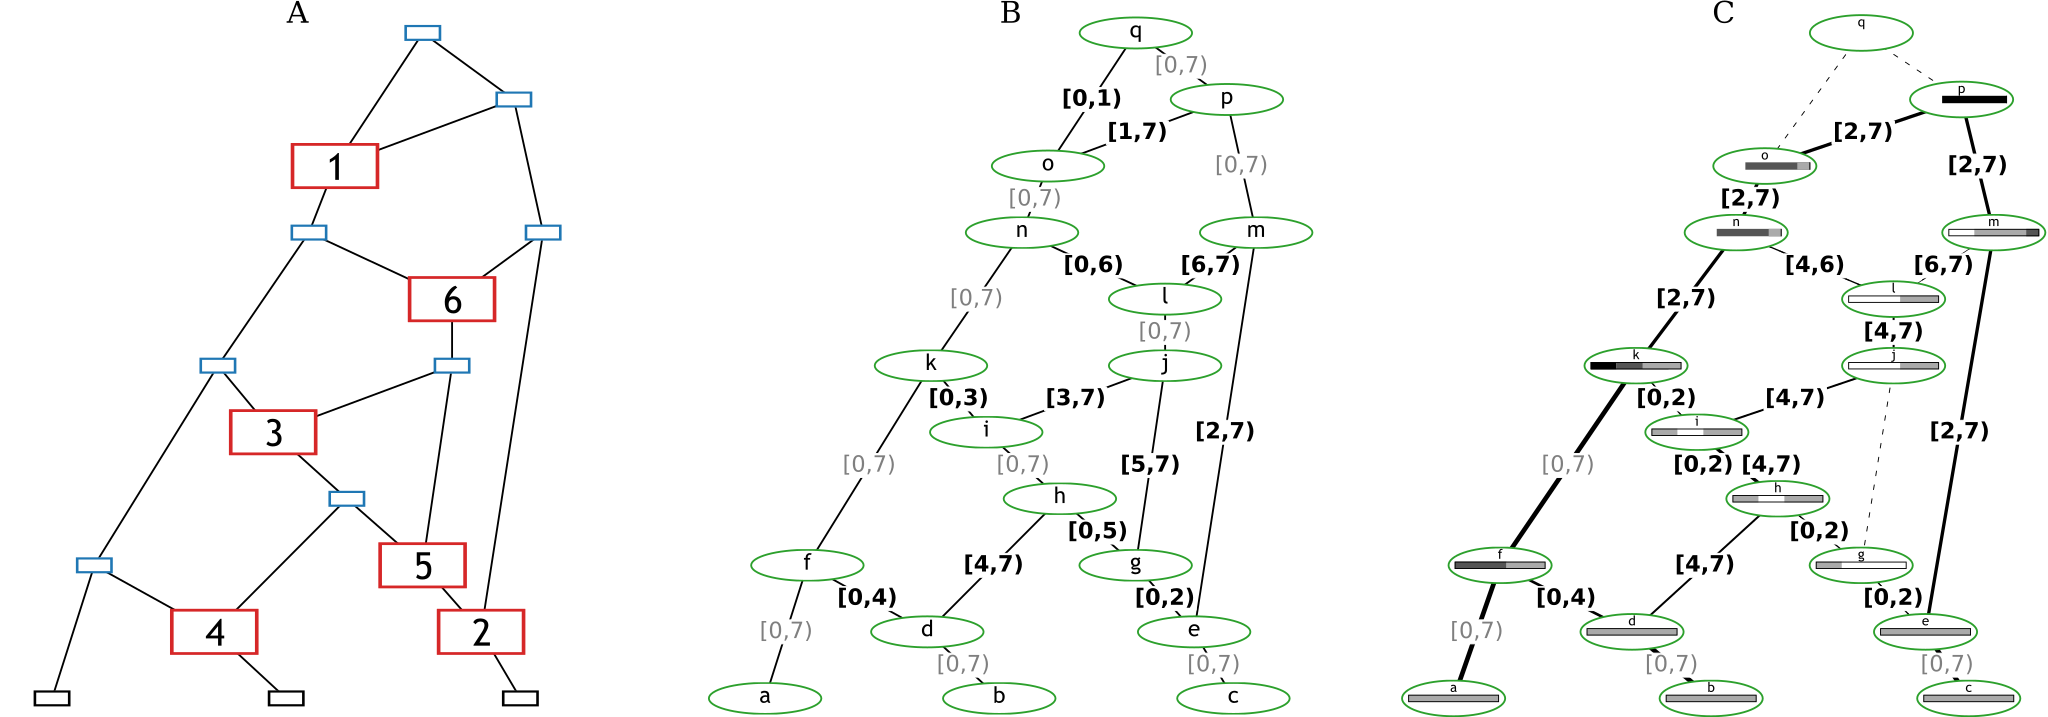
\includegraphics[width=\textwidth]{illustrations/ancestry-resolution}
\caption{\label{fig-ancestry-resolution}
The \citet[][Fig.~1]{wiuf1999recombination} example graph as a gARG,
with contrasting
edge annotation schemes. (A) Immediate edge annotation, reflecting ``local''
transmission of all genetic material between parent and child. All edges span
the full genome from position 0 to 7, apart from those linking a recombinant
and its two parents (bold). (B) Sample-resolved edge annotation: the
Hudson-like simplification algorithm has been used to shorten edge spans to
reflect only the upwards transmission of genetic material from the samples
\textsf{a}, \textsf{b}, and \textsf{c}. The depiction of the genome within each
node is shaded as in Fig.~\ref{fig-arg-in-pedigree}A to show coalescing
regions of genome back to the grand MRCA \textsf{w}. Line widths reflect
the genomic span of each edge, which helps visualise the relative importance of
different transmission pathways.
}
\end{figure}

ARGs are inherently a retrospective structure defined in terms
of a set of sample nodes (usually the leaves), and,
as we discuss in section XXX, storing sample-resolved ancestry
intervals (Fig~\ref{fig-ancestry-resolution}B) is generally much more
useful than storing the local parent-child intervals of inheritance
(Fig~\ref{fig-ancestry-resolution}A).
Indeed, storing local parent-child
inheritance intervals for edges is really only of interest because of
its direct correspondence with the classical approach of associating
breakpoints with recombination nodes in an eARG. The eARG encoding
is simply a more limited form, in which the only types of direct
inheritance we can have are the entire genome, or the intervals
at either side of a recombination breakpoint.

Fig~\ref{fig-ancestry-resolution}A is an instructive example
from the literature \citep{wiuf1999recombination} and illustrates
how a classical eARG can be described as a gARG with local edge annotations
(directly corresponding to the eARG description), and how we can
then derive the ancestry resolved edge annotations.
It is important to note, however, that the example is a sample from
the so-called ``big'' ARG \emph{process} (see Appendix XXX)
and has several features that we are unlikely to infer in practice.
For example, by definition the samples contain no genetic information about
node \textsf{j} and so it is unlike to be inferred.
Likewise, is is unlikely we would have information to infer the ``grand MRCA''
\textsf{w} as all regions of the genome have already reached a
common ancestor separately
(in nodes \textsf{o}, \textsf{u}  and \textsf{v}).

% Third, there exist nodes such as
% \textsf{k} with two children (i.e. ``common ancestor'' nodes in Hudson's terminology)
% but in which no ancestral coalescence occurs. Fourth, some breakpoint positions occur
% within regions of genome that are not ancestral (e.g. the breakpoint at position 3 in
% node \textsf{k}). In this case sample-resolved edge annotations lose the exact position of
% the breakpoint, although they retain the information that a breakpoint occurred between
% positions 2 and 4 (which is sufficient for calculating the likelihood, see appendix XXX).

Given the local inheritance edge annotations
(Fig~\ref{fig-ancestry-resolution}A),
 we obtain the sample-resolved edge annotation
(Fig~\ref{fig-ancestry-resolution}B) by traversing the graph backwards in time
from sample nodes (\textsf{a}, \textsf{b}, \textsf{c}).
Proceeding in topological order (such that an ancestor node is visited
after all of its descendants) the ancestral material for a node is the
union of the ancestral intervals on its inbound edges. We then annotate
the outbound edges with the intersection of their local inheritance and
just-computed ancestral intervals for the node.
For example, node \textsf{d} in Fig~\ref{fig-ancestry-resolution}
carries ancestral material on the interval $(0, 4]$, since it
is the left-hand parent of the recombinant \textsf{b}. The edge
joining \textsf{d} to its ancestor \textsf{h} then carries ancestral
material on $(0, 4]$ since although \textsf{d} inherits the entire interval
$(0, 7]$ from \textsf{h}, only $(0, 4]$ is ancestral to the sample.
This process is directly analogous to Hudson's simulation algorithm
(Appendix XXX).

These alternatives of recording the direct inheritance of genetic material from
parent to child vs the propagation of genomic intervals ancestral to the sample
are analogous to running forwards-time vs backwards-time simulations.
Indeed, the process of taking a graph with edges annotated with direct parent-child
inheritance (Fig~\ref{fig-ancestry-resolution}A) and producing the equivalent
``ancestry resolved'' graph in which only those genomic intervals that are
ancestral to the sample are retained (Fig~\ref{fig-ancestry-resolution}B)
is the same key algorithm underlying recent advances in forwards-time simulation.
\cite{kelleher2018efficient} developed a method in which forwards-time
simulations are performed by recording all parent-child genetic relationships
(i.e.~annotating the edges in the simulated pedigree with the genomic
intervals inherited by a child from a parent) and periodically ``simplifying''
this structure to retain only ancestral relationships that are relevant
to the ancestry of the current population. In many situations, recording
the full genetic ancestry of the population in this way is orders of magnitude faster
than the alternative of tracking
sequences~\citep{kelleher2018efficient,haller2018tree}.


\section*{Precision of ancestry information}
Ancestral recombination graphs are often characterised
as consisting of a complete record of the genetic history
of a sample. For example,
\cite{rasmussen2014genome} state that an ``ARG provides a record of all
coalescence and recombination events since the divergence of the sequences
under study'' and
according to \cite{deng2021distribution} an ARG
``provides all the information about the genealogical history of a sample,
including the locations of recombination events.'' It is worth
questioning, however, whether such comprehensive information
will always be available, and in particular whether our
representation of genealogical history should \emph{require}
such precision. Simulations will usually generate complete
information about the history of a sample, of course, but
we may not have sufficient information to infer such detail.

% Not sure where this goes, but there are some critical points
% that we want to explain and not just throw out there in the
% discussion.
A critical distinction between the eARG and gARG encodings
is the level of precision about the time and location of
recombination events that is required. In an eARG, we are
required to be absolutely precise about every recombination
[explain and contrast with gARG, referring to examples]

% % JK: This is very rough, just jotting down the basic ideas,
% % will need substantial revision.
% It is not clear that such complete information will always
% (or indeed ever) be available from inferences. We may be
% able to precisely identify the location and timing
% of recent recombinations (particularly if detailed pedigree
% information is available) but beyond this, the information
% required simply isn't present. When sampling from a
% process such as the Sequentially Markov
% Coalescent~\citep{mcvean2005approximating,marjoram2006fast}
% like ARGweaver~\citep{rasmussen2014genome}, it is true that
% we do obtain a fully resolved ARG with precise
% information about recombination, but it is reasonable
% to question how much information from the data is used
% to support older recombinations, in particular.

% It is helpful to consider the difference between fully
% resolved binary trees and those that contain polytomies.

% The situation is in fact directly analogous: an ARG that
% contains fully resolved recombination information must have
% at most parents per node.


% At the very least, it is not reasonable for the \emph{data
% structure} to require complete precision in order to
% represent some less precise. This is a fundamental
% advantage of the gARG encoding over the classical eARG
% method: we are not forced to posit a precise cause (recombination
% event) for every effect (difference between adjacent trees).
% These differences in precision of recombination
% information are illustrated in the ARGs estimated by different
% methods, as we see in the next section.


\begin{figure} \begin{center}
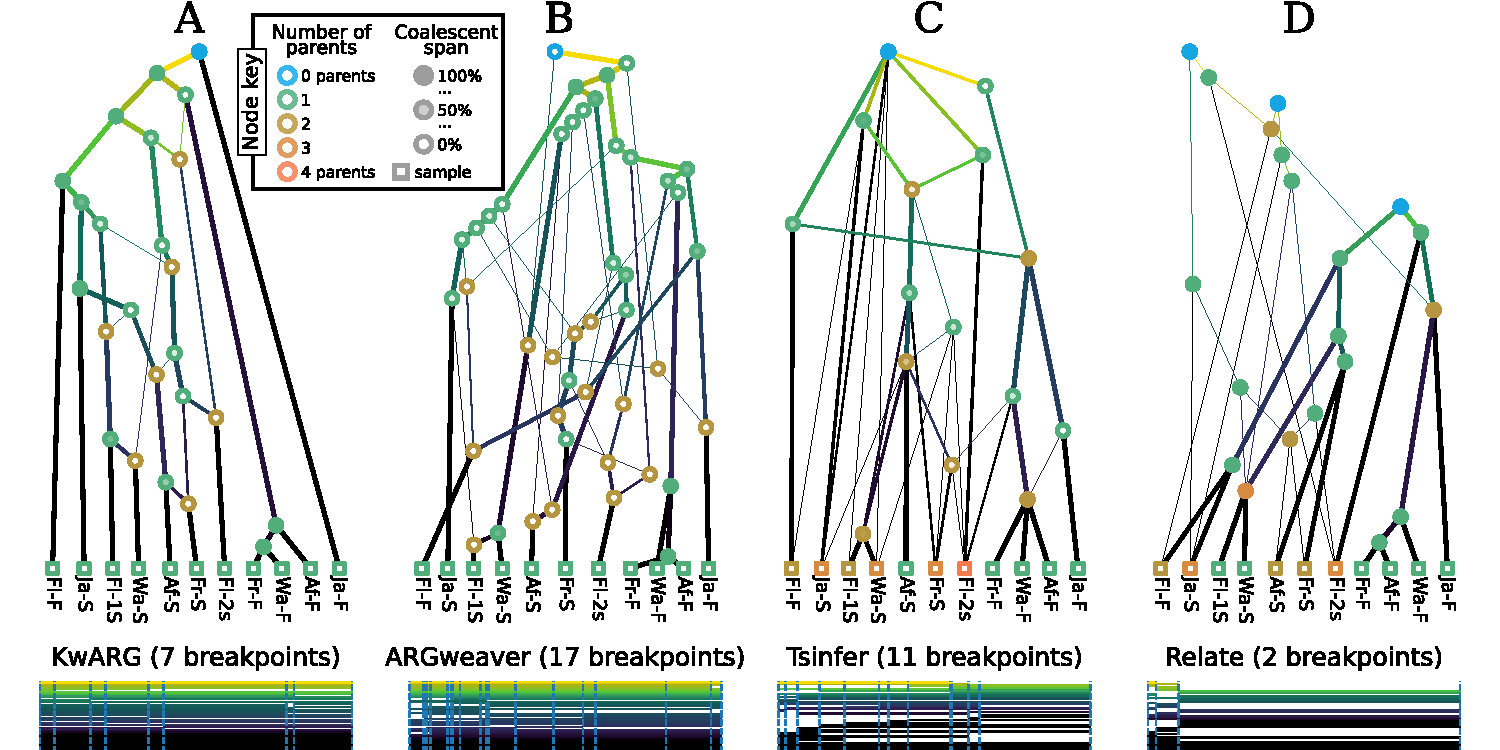
\includegraphics[width=\textwidth]{illustrations/inference.pdf} \end{center}
\caption{\label{fig-inferred-args} ARGs inferred by
(A) \kwarg~\citep{ignatieva2021kwarg},
(B) \argweaver~\citep{rasmussen2014genome,hubisz2020inference},
(C) \tsinfer~\citep{kelleher2019inferring},
and (D) \relate~\citep{speidel2019method}
for 11 samples of a 2.7kb region of the \textit{Drosophila melanogaster} ADH
locus~\citep{kreitman1983nucleotide}. The \argweaver\ example
is a sample from the inferred posterior distribution.
Note that the position of points on the
Y axis is that chosen for graphical clarity by the graphviz \texttt{dot}
algorithm,  rather than being
a direct measure of time. Additional notes about these ARGs.
}
\end{figure}

To illustrate this critical point, we inferred ARGs for the
the classical \citet{kreitman1983nucleotide} benchmark dataset
using four recent inference methods and show the results in
Fig~\ref{fig-inferred-args}.
While there is some consistency among the inferred ARGs (such as the samples
FR-F, WA-F and Af-F being grouped into the same clade), there
are also considerable differences. For this dataset, the minimum number
of recombination breakpoints required in the absence of recurrent mutation
is 7~\citep{song2003parsimonious}, and the number of inferred breakpoints
under the input mutation and recombination rates
varies from 2 (\relate) to 17 (\argweaver).
The ARGs inferred by the different methods also have major differences
in how recombination information is represented. Essentially,
\kwarg\ and \argweaver\ infer a specific causal recombination \emph{event}
for each breakpoint, and those events are fully
described in the output graph. On the other hand, \tsinfer\ and
\relate\ do not infer causal events but instead focus on
representing the inferred \emph{effect}: breakpoints between the
trees. It is important to note that this does not imply that
the methods must then necessarily infer only a sequence of
unrelated local trees
% More? See https://github.com/tskit-dev/what-is-an-arg-paper/issues/38
% for discussion. I'm sure there were other examples of people saying
% that
(as claimed by e.g.~\citep{hejase2020summary}),
and information about recombination and the correlation structure
between trees is not ``all or nothing''.
Both methods capture correlation structure between trees:
\relate\ first infers local tree topologies and then identifies edges
that persist from one tree to the next as a separate step
(in a similar manner to \espalier~\citep{rasmussen2022espalier}), while
\texttt{tsinfer} explicitly constructs nodes that are shared across local
trees.

Because the ARGs inferred by \tsinfer\ and \relate\ do not contain
explicit recombination events we cannot compute a likelihood
under the coalescent with recombination (see appendix XXX).
[Some stuff about whether we should see this as necessary or not,
but maybe we should keep this for the conclusion?]

\section*{ARG simplification}\label{ARG_simplification}

Not all nodes in an ARG are equal. Assuming that we have sequenced the
genomes of the samples, there are intrinsic limits on what can
be known about more ancient nodes, determined by the graph topology
and the flow of ancestral material through it.
\emph{Simplification}~\citep{kelleher2018efficient} is the process
of removing nodes and re-writing edges in a gARG to remove
various types of redundancy, while maintaining the crucial properties
that the ``meaningful'' topology in the local trees is not affected,
and the relationship between nodes in adjacent trees is maintained.

\begin{figure}
\centering
\vspace{5em}
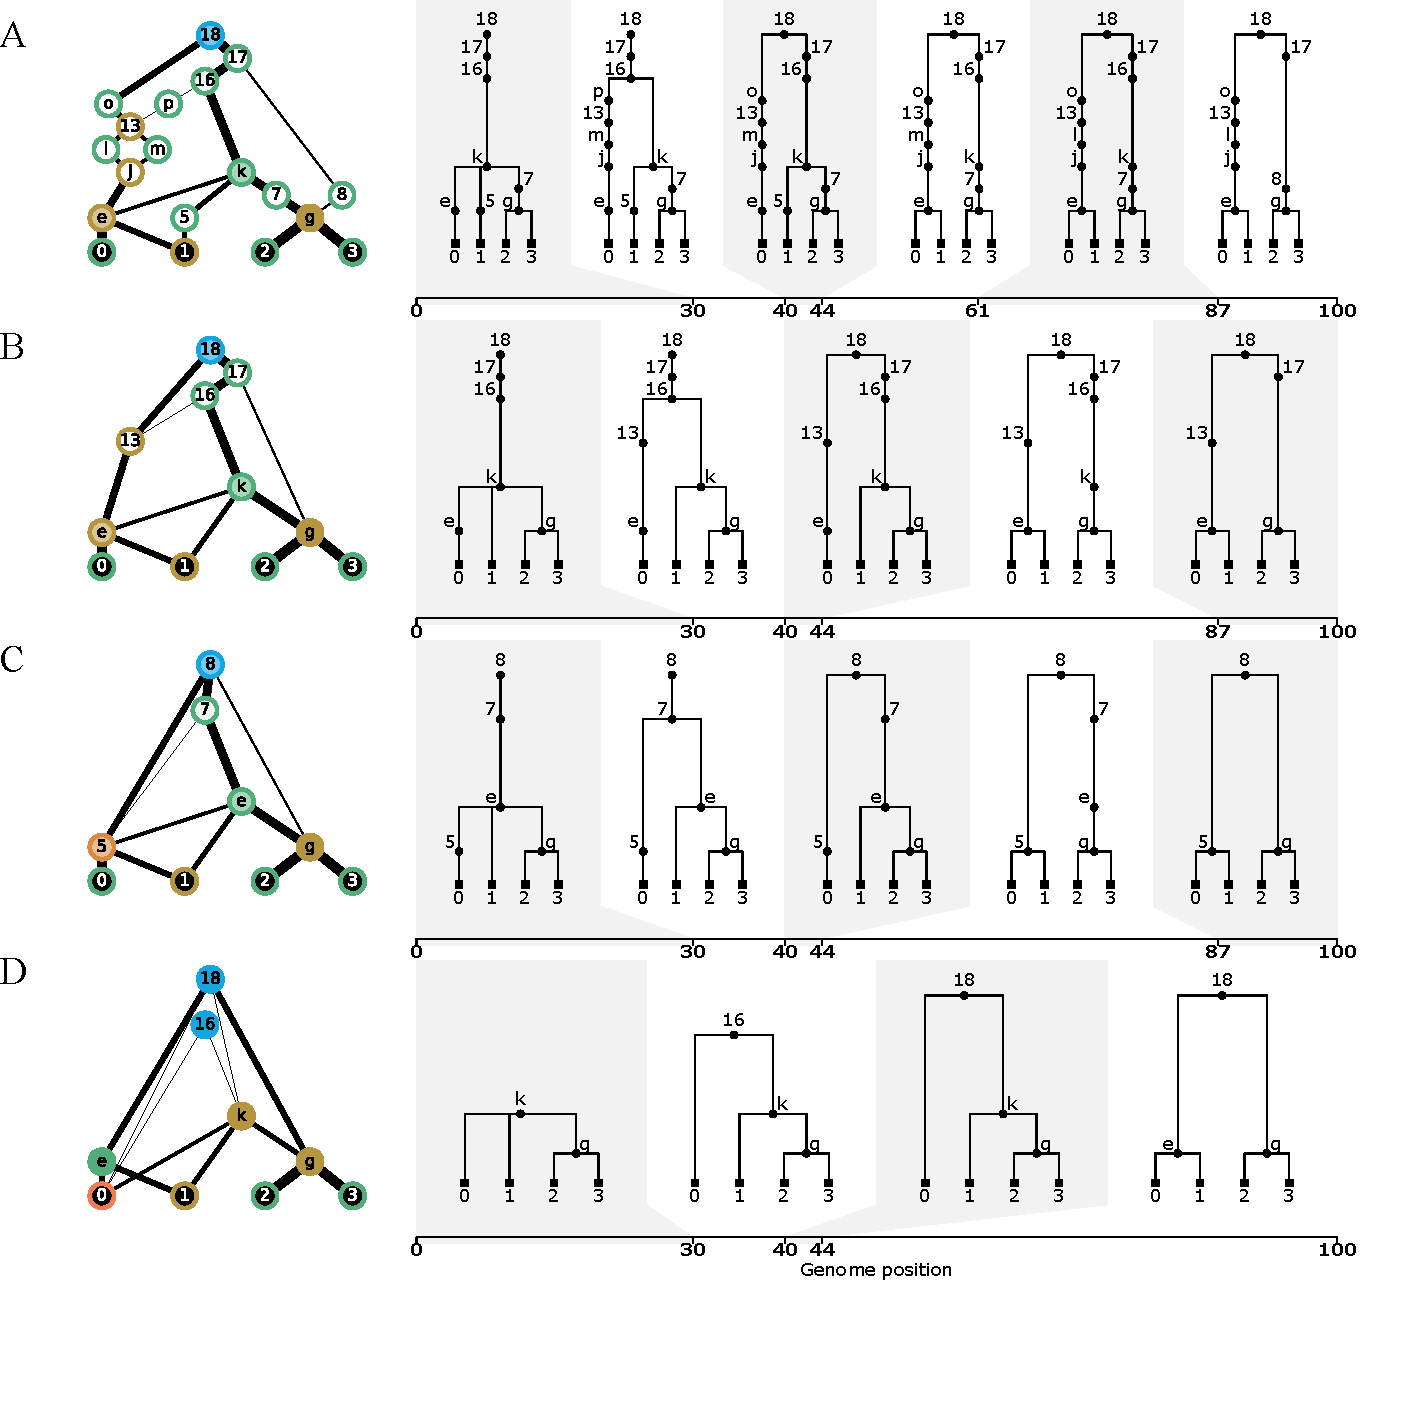
\includegraphics[width=\linewidth]{illustrations/simplification}
\caption{\label{fig-simplification}
ARG simplification. In all cases the graph visualization is shown on the left
and the equivalent marginal trees on the right.
(A) A gARG simulated from a diploid Wright-Fisher
model. Note that the genome \textsf{k} has three children, and the genomes
\textsf{e} and \textsf{g} simultaneously have multiple parents and multiple children;
neither could be directly represented in a Griffiths-like eARG encoding
(see the ``\nameref{eARG}'' section). The penultimate local tree is highlighted to aid discussion.
(B) Simplified to remove all
% trying out this terminology - can define in the text
1-connected graph components (e.g., diamonds such as \textsf{jlnm}).
(C) Remove nodes that are unary in all local trees. This removes both recombinant nodes
that have only one child (e.g. \textsf{n}) and nodes that have more
than one child (i.e. are ``common ancestors'') but never represent coalescences
in the local trees (e.g. \textsf{r}).
(D) Rewrite edges to bypass any unary nodes in local trees. Note that this loses lineage
information such as the fact that \textsf{k} is connected to \textsf{a} via \textsf{e}.
}
\end{figure}

% Q: would it help to talk about ``tree vertices'' here or would it
% just be more confusing? I worry that people would think that
% they are two different things then, and it's really important
% that they get that a node-is-a-node


The ideas of ``meaningful'' local tree topologies revolve around the
presence of ``unary'' nodes: a node in the tree that has exactly
one child. Fig.~\ref{fig-simplification} show a series of successive steps of
simplification, starting with a complete gARG simulated under a
(backwards-time) Wright-Fisher
model, shown both as a graph on the left, and the equivalent set of 6
local trees on the right (Fig.~\ref{fig-simplification}A). Consider the path above node
\textsf{a} in the penultimate tree, highlighted in yellow and covering genomic positions
60 to 70. On this path, before \textsf{a} meets its common ancestor with the other samples at
node \textsf{q}, it passes through  \textsf{e},  \textsf{j},  \textsf{m},  \textsf{n} and
\textsf{p}, which in this region of the genome are all unary nodes. This reflects the
passage of this span of genome through the ARG towards the root (see the
``\nameref{Ancestry_resolution}'' section).
Such unary nodes in a local tree are not usually considered important;
% because they provide little information and are not
% detectable by information from any given individual tree.
nodes usually mark the points where samples find a
 \emph{common} ancestor, such as node \textsf{q} in the highlighted
tree. For many purposes, we would therefore consider a path directly
joining sample \textsf{a} to node \textsf{q} to be of equivalent status to the path
containing the intermediate unary nodes. Simplification is the process of removing
these less informative and (for most computational purposes) inefficient nodes
from the local trees and the corresponding annotated graph.

The first type of simplification that we can perform is to remove
graph topology that is invisible to the samples. The best
known example of such topology is a so-called
``diamond''~\citep{rasmussen2014genome}
in which the two parent nodes of a recombination immediately
join again into a common ancestor (e.g.~\textsf{j}, \textsf{l}, \textsf{m}
and  \textsf{n} in Fig.~\ref{fig-simplification}A).
Unless we are specifically
interested in the recombination event or ancestral genomes,
there is no information in this topology and the diamond can be
replaced by a single edge. More generally, any
subgraph which is singly-connected in both the leafward and
rootward direction (a ``super-diamond'') is non-identifiable and can be
replaced by one edge. This definition includes the case
of a node that has one inbound and one outbound edge, such as
nodes \textsf{f} and \textsf{h}.
Fig.~\ref{fig-simplification}B shows the result of this type of
graph topology simplification.

Simplifying away diamonds will remove many unary nodes from the
local trees, but there can still be nodes that are unary in all
of the local trees. In particular, a node can represent a recombinant
with multiple parents in the graph but only a single child (e.g.\ node \textsf{n}
in Fig.~\ref{fig-simplification}B), or can represent a common ancestor with
multiple children in the graph but in which no local coalescence takes place
(node \textsf{r} in Fig.~\ref{fig-simplification}B).
% point out that this is why Hudson refers to CA nodes, not coalescence nodes
Such nodes are not singly connected in the graph, but are nevertheless unary in
all of the local trees. The operation to remove them,
the results of which are shown in Fig.~\ref{fig-simplification}C,
therefore requires knowledge not just of the graph topology, but also of the
edge annotations. Removal of recombinant nodes can produce graph nodes with
more than 2 parents (e.g.~node \textsf{e}); likewise, removal of
common ancestor but non-coalescent nodes can produce graph nodes with
more than 2 children (e.g.~node \textsf{s}). These represent a ``stacking up'' of
multiple---often indistinguishable---events into a single node,
something which is impossible to encode in an eARG.

% JK: Text moved from an earlier section. See if we want to reuse this here
% if not already said.
% Indeed a single node can have both multiple children
% and multiple parents. This would be the case in Fig~\ref{fig-arg-in-pedigree} if,
% for instance, node \textsf{a} were to have two children.
% % It is a shame that this is not actually shown in fig 3, but I don't think
% % we can do this unless we have 5 generations
% Moreover, a single node can have more than 2 children, and (as we shall see in
% the ``\nameref{ARG_simplification}'' section), more than 2 parents. Another way to
% state this is that transitions between nodes in a gARG can encapsulate multiple
% events in an eARG.


The remaining nodes are MRCAs of some subset of the samples
at \emph{some} positions along the genome. We still have
some unary nodes in the local trees, but these nodes will
correspond to a coalescence in at least one other
local tree. For example, node  \textsf{k} is unary in the second tree
of Fig.~\ref{fig-simplification}C, but is either binary
or ternary in all subsequent trees (recall this is a Wright-Fisher
simulation). The final level of simplification is to alter the edge annotations
such that, although no nodes are removed from the graph, \emph{all}
unary nodes disappear from the local trees (Fig.~\ref{fig-simplification}D).
It is common for this operation to remove nodes above the top MRCA node
in the tree, resulting in many more root nodes (here, \textsf{q} and \textsf{k}
become roots). [And continue]
% Note that although this last stage produces much simpler local trees, by
% removing information about the exact paths taken by lineages through
% the graph, it loses potentially important information about shared edges
% between trees. It is not clear whether (c) or (d) leads to a more compact
% representation of the ARG in terms of number of edges.

\section*{Relationship between ARGs and trees}

We have seen that the local tree for a given position on
the genome can be extracted from an ARG by starting at the
leaves and following the appropriate paths through the graph.
However, this tells us little about the relationship between
adjacent trees, and what the properties of overall ensemble of
local trees are.
A recombination between two adjacent trees causes them to
differ by a ``subtree prune-and-regraft'' (SPR)
% Hein et al call it the ``subtree transfer'' operation but it's
% the same thing.
operation~\citep{hein1990reconstructing,song2003on,song2006properties}.
The number of SPRs required to transform one leaf-labelled tree
into another is known as the SPR distance
% Hein 1996 say that SPR distance is NP-hard, but Allen 2001
% say this is wrong. But then Bordewich went ahead and said
% yes, actually it is NP hard.
and is NP-hard to
compute~\citep{hein1996complexity,allen2001subtree,bordewich2005computational}.

The effects of recombination as we move from left-to-right along
the genome in an unsimplified gARG are easy to interpret.
Consider the highlighted tree in Fig~\ref{fig-simplification}A.
In it the parent of \textsf{e} is \textsf{j}, whereas in the next tree
its parent is \textsf{k}. Since both parents are present as
unary nodes in the tree, we simply change one edge in
order to effect the transition.
% Need revising to fit new example
A more complex transition occurs when we have a regraft operation
that occurs above the current root (i.e., the current oldest
non-unary node). For example, the transition between the
second and third trees corresponds to node D switching
from the path through I to H, and we then must add branches
corresponding to passing through L and meeting at M.

The equivalence between an ARG and a set of local trees
separated by SPRs is often mentioned [e.g. x y z], but
it is important to note that while extracting local
trees from an ARG is straightforward, the converse
process of reconstructing precisely the same ARG from
these trees is more problematic. If the internal
nodes are consistently labelled and unary nodes are
included in the local trees (e.g., Fig~\ref{fig-simplification})
then it is easy to exactly reconstruct the ARG.
Otherwise, the problem is much more difficult and it
may not be possible to uniquely reconstruct the original ARG.
Without labels for the internal nodes, we are forced to
to reason about which subtrees remain the same and which
differ due to the SPR separating adjacent trees in order to
assign node identity. Without the internal unary nodes marking
recombinations, we must infer their existence. In
general, there will not be a unique solution to this problem,
and so there can be many possible ARGs compatible with
a given list of leaf-labelled binary trees.
This is the approach taken by the Espalier inference
method~\citep{rasmussen2022espalier}, which finds a
set of SPRs that reconcile independently inferred
trees from different regions of the genome.

\section*{Computational efficiency}
The succinct tree sequence data structure (usually known as a ``tree sequence''
for brevity, but see later comment on confusion around this point)
is a concrete encoding of a gARG, as discussed in this article.
It was originally developed as part of the \texttt{msprime}
simulator~\cite{kelleher2016efficient} and subsequently ...

[The tree sequence encoding is very efficient for lots of things. Examples]

In retrospect, the choice of terminology was unfortunate, and has led to
significant confusion. [More]



\section*{Discussion}

Discussion points (may or may not be used, certainly would be heavily revised)

\begin{itemize}

\item Recap quickly distinction bewtween aARG and gARG.Then:
    This, coupled with
    the explicit association of genome coordinates with edges, allows
    us to represent even the bewilderingly complex patterns of relatedness
    present in modern datasets.


\item It is unfortunate that we are adding yet another meaning to the
term ARG here, but all we're really doing is making the implicit
assumptions that others have made (i.e., describing the output of
Relate, tsinfer etc as ARGs) and making them concrete. We need to have a
term to describe all of these things, and since people are already using
ARG for this, we might as well make it rigorous. We can then move away
from the unfruitful discussion about which methods infer a ``true'' or
``real'' ARG (none do, really, under the original definitions) and
instead start discussing the \emph{properties} of these ARGs. (See
next point also.)
\item Terminology based around an inferred ancestry being a ``true''
ARG is impoverished and misleading. The only reasonable interpretation
of a ARG being true or not is whether it's a sample from the coalescent.
Most inference methods (and all that scale well) do not. In any case,
the coalescent is just one model, and a highly idealised one. It is
exceedingly unlikely that the actual ARG describing the ancestry
of any biological population is ``true'' ARG in this sense. The terminology is
impoverished because it reduces the possibilities available
to something either being an ARG or not, whereas there are many different
interesting properties of these structures that we should be able to
discuss and compare.
\item tskit can represent any ARG.
\item Interchange is a real problem, and if we're going to realise the
potential for ARGs in genomics we must solve it. Efforts to standardise
phylogenetic networks haven't done very well (~\citep{cardona2008extended}
has 89 citations). The only real effort to standardise an ARG format
based on extending GraphML~\citep{mcgill2013graphml} has 11 citations.
GraphML~\citep{mcgill2013graphml} has some of the same key ideas
as tskit though, in particular allowing the annotation of ``live sites''
to an edge as a set of disjoint intervals that hold ancestral material.

\item There are real computational disadvantages to the Griffiths ARG
data structure. Having two types of node (three really, as we need
``sample'' nodes which are also treated differently) complicates algorithms,
and makes it difficult to reason about the structure of the ARG as a
graph. For example, there's some weirdness about mutations over
recombination nodes discussed by Gusfield [Ana?]

\item Comparison metrics are a problem. All evaluations has essentially
looked at either some form of pairwise comparison of trees along the genome
using tree metrics, or looked at the distributions of TMRCAs. No
one has succeeded in performing any comparisons of ARGs beyond
regarding them as a sequence of independent trees. If we genuinely believe
that ARGs are more than this, then we need to devise some metrics that
consider more than the local tree structure.

\item Throughout, we considered ARGs defined for a single chromosome comprising
of a fixed number of discrete sites. Our argument applies equally well to ARGs
defined for several non-homologous chromosomes \citep{fearnhead2003ancestral,
koskela2019robust} and to idealised, continuous chromosomes.

\item The gARG structure as described here is sufficiently expressive
to model any form of homologous genetic transmission between individuals,
and is far more flexible than the classical eARG approach.
Phylogenetic networks~\citep{huson2010phylogenetic} are a more
general concept, and specific classes capture dynamics that
cannot be modelled using an ARG. For example,
reassortment networks model the exchange of
(non-recombining) genomic segments between viral particles inside a co-infected host,
and hybridisation networks, model the genetic material from
different species combining to create a hybrid.
Similarly Genome Graphs~\cite{novak2017genome} model complicated things
within species. Future work should look to capture all of these things
in a single structure.

\end{itemize}


% TODO not clear this belongs in the discussion, but we'll definitely
% want to make some of these points, even if they are being repeated
% from earlier section.
It is difficult to imagine a practical calculation performed on an
ARG that does not involve either the sequential generation of trees
along the genome or the resolved ancestry segments.
Knowing the resolved segments in an ancestry resolved gARG allows
us to perform many calculations without explicitly generating
the trees, and lets us work with the ancestry on a genome-by-genome
basis. We give three examples here. Firstly, generating mutations
on edges can be performed very quickly on an ancestry resolved
gARG, since we only need to examine $O(|E|)$ edges rather than
$O(nt)$ tree branches (assuming $n$ samples and $t$ marginal trees)
~\citep{baumdicker2021efficient}. If the ancestry were not resolved,
we would generate a large number of mutations on areas of the edge that
are non-ancestral. Secondly, computing the likelihood of a given
ARG realisation under the coalescent with recombination model
requires that we essentially recapitulate the state of Hudson's
algorithm (see XXX section) at each node in
the graph~\citep{baumdicker2021efficient}. Having resolved ancestry
substantially simplifies this process. Thirdly, computing
[FIXME describe what we did in tsdate]~\citep{wohns2022unified}.

Sequentially generating the marginal trees along the genome
is also fundamental, and is necessary whenever we need to
perform calculations that are contingent on more than just the
isolated properties of an edge. \cite{kelleher2016efficient}
showed how all trees can be sequentially generated in
constant time per tree transition in a fully simplified gARG.
Furthermore, we can easily reason about how tree topologies
change (and stay the same), leading to efficient algorithms
for computing population genetic
statistics~\citep{kelleher2016efficient,kelleher2018efficient},
implementing the Li and Stephens
model~\citep{kelleher2019inferring,wohns2022unified}
and likely many more.


\bibliographystyle{plainnat}
\bibliography{paper}

\setcounter{secnumdepth}{2} % Print out appendix section numbers

\appendix
\section*{Appendix}

\subsection*{The Big and Little ARG}
\label{app-big-and-little-arg}

Here we review the two predominant stochastic processes which construct ARGs:
the ``big" ARG process of \cite{griffiths1997ancestral}, and the ``little" ARG process of
 \cite{hudson1983properties}. The big ARG process is mathematically simpler
 but is computationally intractable due to generating a vast number of ancestors
 which contribute no genetic material to the initial sample.
The little ARG process avoids non-genetic ancestors at the cost of more complex
dynamics and state space. We also demonstrate that evaluating the sampling probability
of either process---a key quantity in many statistical approaches---requires that the
gARG (or eARG) data structure be interpreted in a model-specific way.

A generic state of the little ARG process consists of a finite collection of lineages $L$,
each of which is a list of disjoint ancestry segments $(\ell, r, a)$, where
$[\ell, r)$ is a half-closed genomic interval and $a$ is an integer
tracking the number of samples to which the lineage is ancestral over that interval.
We also usually track the node associated with each segment, but
that is not important for our purposes here so we omit it to lighten notation.
The initial condition for a sample of $n$ genomes of length $m$ consists of $n$ lineages
of the form $\{(0, m, 1)\}$. The process traverses a series of common ancestor and
recombination events backwards in time.
Recombination events happen at rate $\rho \nu / (m - 1)$,
where $\rho \geq 0$ is a per-genome recombination rate and
 \[
 \nu = \sum_{x \in L}\left( \max_{(\ell, r, a) \in x}r
     - \min_{(\ell, r, a) \in x}\ell - 1 \right)
 \]
 is the number of available ``links" surrounded by ancestral material.
 At a recombination event we choose one of these links uniformly and break it,
 replacing the original lineage in $L$ with two new lineages containing the ancestral material
 to the left and right of the break point, respectively.

Common ancestor events occur at rate $\binom{|L|}{2}$.
In a common ancestor event, two uniformly sampled lineages have their segments
merged into a single ancestor lineage, which is added to $L$.
If the lineages have overlapping intervals of ancestry,
say, $(\ell, r, a_1)$ and $(\ell, r, a_2)$, a
\emph{coalescence} occurs. The result is a segment
$(\ell, r, a_1 + a_2)$, and if $a_1 + a_2 < n$ it is included in the
ancestor lineage. Otherwise, if $a_1 + a_2 = n$, we have found
the most recent common ancestor of all samples in the interval$[\ell, r)$
and do not need to simulate its history any further.
Non-overlapping intervals from the two lineages are included
 in the ancestor lineage without changes. Eventually,
we find resultant lineages in which all segments have fully coalesced,
and so the number of extant lineages gradually falls to zero.

In the Griffiths formulation (the big ARG process), each edge in the graph corresponds to an extant
lineage and nodes are events in the process. The $n$ initial leaf nodes are
sampling events. Common ancestor events occur at rate $\binom{|L|}{2}$.
When a common ancestor event happens, two uniformly chosen lineages
merge into a common ancestor lineage.
Recombination events happen at rate $|L| \rho$. Here, we choose a lineage (i.e.\ edge) uniformly,
and a breakpoint $0 < x < m$ uniformly on its genome. We terminate the edge at a
node, record the breakpoint, and start two new edges from this node. The process
then continues until there is only one lineage left (the Grand Most Recent
Common Ancestor, GMRCA), which is guaranteed to
happen in finite time because of the linear rate of coalescing vs.\ quadratic rate of branching.

The state-space of the big ARG process is much simpler than that of the little ARG process,
which greatly facilitates mathematical reasoning. This simplicity comes at a
substantial cost, however, if we wish to use it as a practical means of
simulating recombinant ancestries.
The number of events in the big ARG all the way back to the GMRCA
is $O(e^\rho)$~\citep{griffiths1997ancestral}, whereas the number
of events required to simulate the little ARG is
$O(\rho^2)$~\citep{hein2004gene,baumdicker2021efficient}.
This disparity arises because the majority of the events in the big ARG are
recombination events which occur outside of ancestral material,
and this do not have any bearing on the ancestry of the initial sample.
Because we don't keep track of the distribution of ancestral material during the process,
we generate a vastly larger graph.

Figure \ref{hudson_vs_bigARG} illustrates the more complex state space
of the little ARG process, as well as the extra events which occur in the big ARG process.
Moreover, it depicts the rates of common ancestors and recombination events in each
interval of time of the realisations.
In order to evaluate these rates, and hence the sampling probability
(see e.g.\ \cite[Equation (3)]{mahmoudi2022bayesian}),
it is necessary to know the number of lineages and number of extant links
available for recombination in each time interval.
This information cannot be recovered from the gARG encoding depicted in
e.g.\ Figure \ref{fig-ancestry-resolution}.
For example, it is clear that a recombination takes place between nodes \textsf{b} and
\textsf{d} as well as \textsf{e}, but the exact time of the event is ambiguous,
and thus so is the number of lineages during the time interval.
Conventions can be introduced to resolve such ambiguities;
for the likelihood-based inference algorithms for the coalescent with recombination,
the two parent nodes are typically created at the time of the recombination event.
See the appendix of \cite{baumdicker2021efficient} for details of evaluating
coalescent with recombination likelihoods using this convention.
This is also the interpretation depicted in
Figure \ref{hudson_vs_bigARG}, but it means that the two edges above node \textsf{b}
in Figure \ref{fig-ancestry-resolution} should correspond to only one lineage,
along which all $m-1$ links are available for recombination.
The lineage then splits into two at the time of nodes \textsf{d} and \textsf{e}.
Nodes \textsf{k}, \textsf{l}, and \textsf{m} in Figure \ref{fig-ancestry-resolution}
demonstrate that the same issue can affect the number of links available for recombination:
without an external convention, the exact time at which the trapped ancestral material on
node \textsf{k} ceases to be available for an effective recombination in the little ARG process.

\begin{figure}[ht]
\centering
% FIXME this is a quick nasty hack to make the figure a bit smaller and
% prevent flushing all the other figures to the end of the document.
\scalebox{0.54}{
\begin{tabular}{cc}
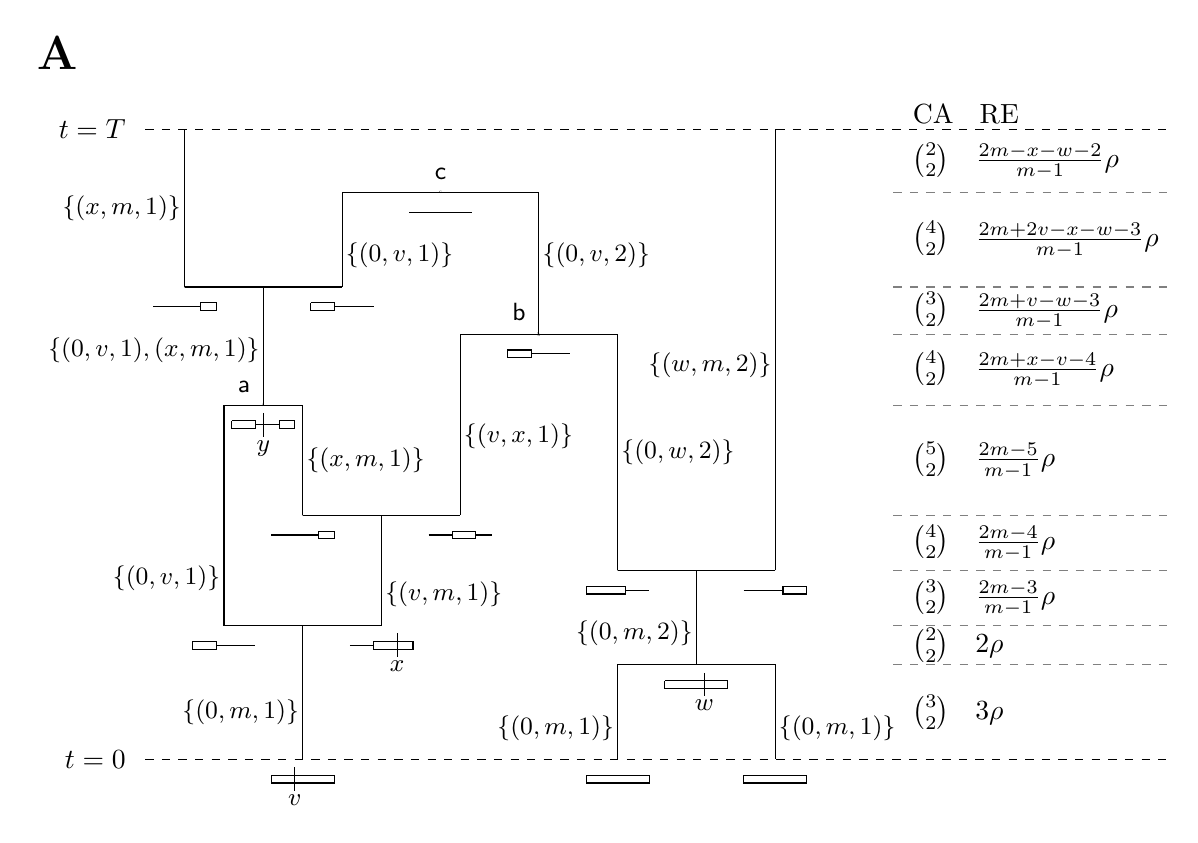
\begin{tikzpicture}
	\node [anchor=north west] at (-3.5,9.3) {\LARGE \textbf{A}};
	\draw (-0.4, -0.2) -- (0.4, -0.2) -- (0.4, -0.3) -- (-0.4, -0.3) -- (-0.4, -0.2);
	\draw (-0.1, -0.1) -- (-0.1, -0.4);
	\node [label=below:{\small $v$}] at (-0.1, -0.2) {};
	\draw (3.6, -0.2) -- (4.4, -0.2) -- (4.4, -0.3) -- (3.6, -0.3) -- (3.6, -0.2);
	\draw (5.6, -0.2) -- (6.4, -0.2) -- (6.4, -0.3) -- (5.6, -0.3) -- (5.6, -0.2);

	\draw (4,0) -- (4, 1.2) -- (6, 1.2) -- (6,0);
	\draw (4.6, 1) -- (5.4, 1) -- (5.4, 0.9) -- (4.6, 0.9) -- (4.6, 1);
	\draw (5.1, 1.1) -- (5.1, 0.8);
	\node [label=below:{\small $w$}] at (5.1, 1) {};

	\draw (0, 0) -- (0, 1.7) -- (-1,1.7) -- (1,1.7);
	\draw (-1.4, 1.5) -- (-1.1, 1.5) -- (-1.1, 1.4) -- (-1.4, 1.4) -- (-1.4, 1.5);
	\draw (-1.1, 1.45) -- (-0.6, 1.45);
	\draw (0.6, 1.45) -- (0.9, 1.45);
	\draw (0.9, 1.5) -- (1.4, 1.5) -- (1.4, 1.4) -- (0.9, 1.4) -- (0.9, 1.5);
	\draw (1.2, 1.6) -- (1.2, 1.3);
	\node [label=below:{\small $x$}] at (1.2, 1.5) {};

	\draw (5, 1.2) -- (5, 2.4) -- (4,2.4) -- (6,2.4);
	\draw (3.6, 2.2) -- (4.1, 2.2) -- (4.1, 2.1) -- (3.6, 2.1) -- (3.6, 2.2);
	\draw (4.1, 2.15) -- (4.4, 2.15);
	\draw (5.6, 2.15) -- (6.1, 2.15);
	\draw (6.1, 2.2) -- (6.4, 2.2) -- (6.4, 2.1) -- (6.1, 2.1) -- (6.1, 2.2);

	\draw (1, 1.7) -- (1, 3.1) -- (0,3.1) -- (2,3.1);
	\draw (-0.4, 2.85) -- (0.2, 2.85);
	\draw (0.2, 2.9) -- (0.4, 2.9) -- (0.4, 2.8) -- (0.2, 2.8) -- (0.2, 2.9);
	\draw (1.6, 2.85) -- (1.9, 2.85);
	\draw (1.9, 2.9) -- (2.2, 2.9) -- (2.2, 2.8) -- (1.9, 2.8) -- (1.9, 2.9);
	\draw (2.2, 2.85) -- (2.4, 2.85);

	\draw (-1, 1.7) -- (-1, 4.5) -- (0,4.5) -- (0,3.1);
	\node [scale=0.2,label=above left:{\small \textsf{a}}] at (-0.5,4.5) {a};
	\draw (-0.9, 4.3) -- (-0.6, 4.3) -- (-0.6, 4.2) -- (-0.9, 4.2) -- (-0.9, 4.3);
	\draw (-0.6, 4.25) -- (-0.3, 4.25);
	\draw (-0.3, 4.3) -- (-0.1, 4.3) -- (-0.1, 4.2) -- (-0.3, 4.2) -- (-0.3, 4.3);
	\draw (-0.5, 4.4) -- (-0.5, 4.1);
	\node [label=below:{\small $y$}] at (-0.5, 4.3) {};

	\draw (4,2.4) -- (4,5.4) -- (2,5.4) -- (2,3.1);
	\node [scale=0.2,label=above left:{\small \textsf{b}}] at (3,5.4) {b};
	\draw (2.6, 5.2) -- (2.9, 5.2) -- (2.9, 5.1) -- (2.6, 5.1) -- (2.6, 5.2);
	\draw (2.9, 5.15) -- (3.4, 5.15);

	\draw (-0.5, 4.5) -- (-0.5, 6) -- (-1.5,6) -- (0.5,6);
	\draw (-1.9, 5.75) -- (-1.3, 5.75);
	\draw (-1.3, 5.8) -- (-1.1, 5.8) -- (-1.1, 5.7) -- (-1.3, 5.7) -- (-1.3, 5.8);
	\draw (0.1, 5.8) -- (0.4, 5.8) -- (0.4, 5.7) -- (0.1, 5.7) -- (0.1, 5.8);
	\draw (0.4, 5.75) -- (0.9, 5.75);

	\draw (0.5, 6) -- (0.5, 7.2) -- (3,7.2) -- (3,5.4);
	\node [scale=0.2,label=above:{\small \textsf{c}}] at (1.75,7.2) {c};
	\draw (1.35, 6.95) -- (2.15, 6.95);

	\draw (-1.5, 6) -- (-1.5, 8);
	\draw (6, 2.4) -- (6, 8);

	% Edge annotations above each event
	\node [label=left:{\small$\{(0,m,1)\}$}] at (0.2,0.6) {};
	\node [label=left:{\small$\{(0,m,1)\}$}] at (4.2,0.4) {};
	\node [label=right:{\small$\{(0,m,1)\}$}] at (5.8,0.4) {};
	\node [label=left:{\small$\{(0,m,2)\}$}] at (5.2,1.6) {};
	\node [label=left:{\small$\{(0,v,1)\}$}] at (-0.8,2.3) {};
	\node [label=right:{\small$\{(v,m,1)\}$}] at (0.8,2.1) {};
	\node [label=right:{\small$\{(0,w,2)\}$}] at (3.8,3.9) {};
	\node [label=left:{\small$\{(w,m,2)\}$}] at (6.2,5) {};
	\node [label=right:{\small$\{(x,m,1)\}$}] at (-0.2,3.8) {};
	\node [label=right:{\small$\{(v,x,1)\}$}] at (1.8,4.1) {};
	\node [label=left:{\small$\{(0,v,1), (x,m,1)\}$}] at (-0.3,5.2) {};
	\node [label=right:{\small$\{(0,v,2)\}$}] at (2.8,6.4) {};
	\node [label=left:{\small$\{(x,m,1)\}$}] at (-1.3,7) {};
	\node [label=right:{\small$\{(0,v,1)\}$}] at (0.3,6.4) {};

	% Dashed lines for start and end times
	\draw[dashed] (-2, 0) -- (11, 0);
	\node [label=left:{$t = 0$}] at (-2,0) {};
	\draw[dashed] (-2, 8) -- (11, 8);
	\node [label=left:{$t = T$}] at (-2,8) {};

	% Numbers of extant ancestors and links, from top to bottom
	\node[label=right:{CA \; RE}] at (7.5, 8.2) {};
	\node[label=right:{$\binom{2}{2}$ \; $\frac{2 m - x - w - 2}{m - 1} \rho$}] at (7.5, 7.6) {};
	\node[label=right:{$\binom{4}{2}$ \; $\frac{2 m + 2 v - x - w - 3}{m - 1} \rho$}] at (7.5, 6.6) {};
	\node[label=right:{$\binom{3}{2}$ \; $\frac{2 m + v - w - 3}{m - 1} \rho$}] at (7.5, 5.7) {};
	\node[label=right:{$\binom{4}{2}$ \; $\frac{2 m + x - v - 4}{m - 1} \rho$}] at (7.5, 4.95) {};
	\node[label=right:{$\binom{5}{2}$ \; $\frac{2 m - 5}{m - 1} \rho$}] at (7.5, 3.8) {};
	\node[label=right:{$\binom{4}{2}$ \; $\frac{2 m - 4}{m -1} \rho$}] at (7.5, 2.75) {};
	\node[label=right:{$\binom{3}{2}$ \; $\frac{2 m - 3}{m - 1} \rho$}] at (7.5, 2.05) {};
	\node[label=right:{$\binom{2}{2}$ \; $2 \rho$}] at (7.5, 1.45) {};
	\node[label=right:{$\binom{3}{2}$ \; $3 \rho$}] at (7.5, 0.6) {};

	% Gray dashed lines to visually separate holding times
	\draw[color=gray, dashed] (7.5, 1.2) -- (11, 1.2);
	\draw[color=gray, dashed] (7.5, 1.7) -- (11, 1.7);
	\draw[color=gray, dashed] (7.5, 2.4) -- (11, 2.4);
	\draw[color=gray, dashed] (7.5, 3.1) -- (11, 3.1);
	\draw[color=gray, dashed] (7.5, 4.5) -- (11, 4.5);
	\draw[color=gray, dashed] (7.5, 5.4) -- (11, 5.4);
	\draw[color=gray, dashed] (7.5, 6) -- (11, 6);
	\draw[color=gray, dashed] (7.5, 7.2) -- (11, 7.2);
\end{tikzpicture}
&
\begin{tikzpicture}
	\node [anchor=north west] at (-3.5,9.3) {\LARGE \textbf{B}};
	\draw (-0.4, -0.2) -- (0.4, -0.2) -- (0.4, -0.3) -- (-0.4, -0.3) -- (-0.4, -0.2);
	\draw (-0.1, -0.1) -- (-0.1, -0.4);
	\node [label=below:{\small $v$}] at (-0.1, -0.2) {};
	\draw (3.6, -0.2) -- (4.4, -0.2) -- (4.4, -0.3) -- (3.6, -0.3) -- (3.6, -0.2);
	\draw (5.6, -0.2) -- (6.4, -0.2) -- (6.4, -0.3) -- (5.6, -0.3) -- (5.6, -0.2);

	\draw (4,0) -- (4, 1.2) -- (6, 1.2) -- (6,0);
	\draw (4.6, 1) -- (5.4, 1) -- (5.4, 0.9) -- (4.6, 0.9) -- (4.6, 1);
	\draw (5.1, 1.1) -- (5.1, 0.8);
	\node [label=below:{\small $w$}] at (5.1, 1) {};

	\draw (0, 0) -- (0, 1.7) -- (-1,1.7) -- (1,1.7);
	\draw (-1.4, 1.5) -- (-1.1, 1.5) -- (-1.1, 1.4) -- (-1.4, 1.4) -- (-1.4, 1.5);
	\draw (-1.1, 1.45) -- (-0.6, 1.45);
	\draw (0.6, 1.45) -- (0.9, 1.45);
	\draw (0.9, 1.5) -- (1.4, 1.5) -- (1.4, 1.4) -- (0.9, 1.4) -- (0.9, 1.5);
	\draw (1.2, 1.6) -- (1.2, 1.3);
	\node [label=below:{\small $x$}] at (1.2, 1.5) {};

	\draw (5, 1.2) -- (5, 2.4) -- (4,2.4) -- (6,2.4);
	\draw (3.6, 2.2) -- (4.1, 2.2) -- (4.1, 2.1) -- (3.6, 2.1) -- (3.6, 2.2);
	\draw (4.1, 2.15) -- (4.4, 2.15);
	\draw (5.6, 2.15) -- (6.1, 2.15);
	\draw (6.1, 2.2) -- (6.4, 2.2) -- (6.4, 2.1) -- (6.1, 2.1) -- (6.1, 2.2);
	\draw [color=red](5.8, 2.3) -- (5.8, 2.0);
	\node [label={[red]below:{\small $z$}}] at (5.8, 2.1) {};

	\draw (1, 1.7) -- (1, 3.1) -- (0,3.1) -- (2,3.1);
	\draw (-0.4, 2.85) -- (0.2, 2.85);
	\draw (0.2, 2.9) -- (0.4, 2.9) -- (0.4, 2.8) -- (0.2, 2.8) -- (0.2, 2.9);
	\draw (1.6, 2.85) -- (1.9, 2.85);
	\draw (1.9, 2.9) -- (2.2, 2.9) -- (2.2, 2.8) -- (1.9, 2.8) -- (1.9, 2.9);
	\draw (2.2, 2.85) -- (2.4, 2.85);

	\draw (-1, 1.7) -- (-1, 4.5) -- (0,4.5) -- (0,3.1);
	\draw (-0.9, 4.3) -- (-0.6, 4.3) -- (-0.6, 4.2) -- (-0.9, 4.2) -- (-0.9, 4.3);
	\draw (-0.6, 4.25) -- (-0.3, 4.25);
	\draw (-0.3, 4.3) -- (-0.1, 4.3) -- (-0.1, 4.2) -- (-0.3, 4.2) -- (-0.3, 4.3);
	\draw (-0.5, 4.4) -- (-0.5, 4.1);
	\node [label=below:{\small $y$}] at (-0.5, 4.3) {};

	\draw (6, 2.4) -- (6, 3.8) -- (7, 3.8);
	\draw [color=red](6, 3.8) -- (5, 3.8);
	\draw (4.6, 3.55) -- (5.4, 3.55);
	\draw (6.6, 3.55) -- (7.1, 3.55);
	\draw (7.1, 3.6) -- (7.4, 3.6) -- (7.4, 3.5) -- (7.1, 3.5) -- (7.1, 3.6);

	\draw (4,2.4) -- (4,5.4) -- (2,5.4) -- (2,3.1);
	\draw (2.6, 5.2) -- (2.9, 5.2) -- (2.9, 5.1) -- (2.6, 5.1) -- (2.6, 5.2);
	\draw (2.9, 5.15) -- (3.4, 5.15);

	\draw (-0.5, 4.5) -- (-0.5, 6) -- (-1.5,6) -- (0.5,6);
	\draw (-1.9, 5.75) -- (-1.3, 5.75);
	\draw (-1.3, 5.8) -- (-1.1, 5.8) -- (-1.1, 5.7) -- (-1.3, 5.7) -- (-1.3, 5.8);
	\draw (0.1, 5.8) -- (0.4, 5.8) -- (0.4, 5.7) -- (0.1, 5.7) -- (0.1, 5.8);
	\draw (0.4, 5.75) -- (0.9, 5.75);

	\draw [color=red](5, 3.8) -- (5, 6.6) -- (4, 6.6);
	\draw (4,6.6) -- (3,6.6) -- (3, 5.4);
	\draw (3.6, 6.4) -- (3.9, 6.4) -- (3.9, 6.3) -- (3.6, 6.3) -- (3.6, 6.4);
	\draw (3.9, 6.35) -- (4.4, 6.35);

	\draw (0.5, 6) -- (0.5, 7.2) -- (4,7.2) -- (4,6.6);
	\draw (1.85, 6.95) -- (2.65, 6.95);

	\draw (-1.5, 6) -- (-1.5, 8);
	\draw [color=red](2.25, 7.2) -- (2.25, 8);
	\draw (7, 3.8) -- (7, 8);

	% Dashed lines for start and end times
	\draw[dashed] (-2, 0) -- (9.1, 0);
	\node [label=left:{$t = 0$}] at (-2,0) {};
	\draw[dashed] (-2, 8) -- (9.1, 8);
	\node [label=left:{$t = T$}] at (-2,8) {};

	% Numbers of extant ancestors and links, from top to bottom
	\node[label=right:{CA \; RE}] at (7.5, 8.2) {};
	\node[label=right:{$\binom{3}{2}$ \; $3 \rho$}] at (7.5, 7.6) {};
	\node[label=right:{$\binom{4}{2}$ \; $4 \rho$}] at (7.5, 6.9) {};
	\node[label=right:{$\binom{5}{2}$ \; $5 \rho$}] at (7.5, 6.3) {};
	\node[label=right:{$\binom{4}{2}$ \; $4 \rho$}] at (7.5, 5.7) {};
	\node[label=right:{$\binom{5}{2}$ \; $5 \rho$}] at (7.5, 4.95) {};
	\node[label=right:{$\binom{6}{2}$ \; $6 \rho$}] at (7.5, 4.15) {};
	\node[label=right:{$\binom{5}{2}$ \; $5 \rho$}] at (7.5, 3.45) {};
	\node[label=right:{$\binom{4}{2}$ \; $4 \rho$}] at (7.5, 2.75) {};
	\node[label=right:{$\binom{3}{2}$ \; $3 \rho$}] at (7.5, 2.05) {};
	\node[label=right:{$\binom{2}{2}$ \; $2 \rho$}] at (7.5, 1.45) {};
	\node[label=right:{$\binom{3}{2}$ \; $3 \rho$}] at (7.5, 0.6) {};

	% Gray dashed lines to visually separate holding times
	\draw[color=gray, dashed] (7.5, 1.2) -- (9.1, 1.2);
	\draw[color=gray, dashed] (7.5, 1.7) -- (9.1, 1.7);
	\draw[color=gray, dashed] (7.5, 2.4) -- (9.1, 2.4);
	\draw[color=gray, dashed] (7.5, 3.1) -- (9.1, 3.1);
	\draw[color=gray, dashed] (7.5, 3.8) -- (9.1, 3.8);
	\draw[color=gray, dashed] (7.5, 4.5) -- (9.1, 4.5);
	\draw[color=gray, dashed] (7.5, 5.4) -- (9.1, 5.4);
	\draw[color=gray, dashed] (7.5, 6) -- (9.1, 6);
	\draw[color=gray, dashed] (7.5, 6.6) -- (9.1, 6.6);
	\draw[color=gray, dashed] (7.5, 7.2) -- (9.1, 7.2);
\end{tikzpicture}
\end{tabular}
}
\caption{(A)
A realisation of the graph traversed by Hudson's algorithm started from a
sample of three chromosomes of length $m$ at time $t = 0$, and
propagated until time $T$. The MRCA on the genetic interval $[v, w)$ is reached
at event \textsf{b}, while that on $[0, v)$ is reached at event \textsf{c}.
The non-ancestral segment $[v, w)$ above
A contributes to the rate of effective recombinations because it
is trapped between ancestral segments. The two columns titled CA and RE
are the respective rates of mergers and recombinations when
the recombination rate is $\rho$.
(B) A corresponding realisation of a big ARG, which augments Hudson's algorithm
by tracking nonancestral lineages. The result is a simpler state space and
dynamics, at the cost of extra nodes and edges, highlighted in red, which do
not affect the local tree at any site.}
\label{hudson_vs_bigARG}
\end{figure}

% Full quote:
% This process simplifies mathematics on the account that the notion of an
% ancestor will have a less restrictive meaning than usual:
% An ``ancestral'' sequence in the birth and death process
% need not have any genetic material in common with a
% sequence descended from it.

\subsection*{Survey of ARG inference methods}

The problem of reconstructing ARGs for samples of recombining sequences has
been of interest since the ARG was first defined. Early methods focused on
finding \emph{parsimonious} ARGs, i.e.\ those with a minimal number of
recombination events \citep{hein1990reconstructing}. Two main approaches
emerged: \emph{backwards-in-time} \citep{lyngso2005minimum} and
\emph{along-the-genome} \citep{song2003parsimonious, song2005constructing}. The
former starts with a data matrix and reduces it to an empty matrix through row
and column operations corresponding to coalescence, mutation, and recombination
events, which construct an ARG from the bottom up. The latter begins from an
initial local tree at a single focal site. Moving the focal site along the
genome changes the local tree via a \emph{subtree prune and regraft} (SPR)
operation whenever a recombination is encountered. Methods based the
backwards-in-time approach are described by \citet{song2005efficient,
wu2008association, thao2019hybrid, ignatieva2021kwarg}, while
\citet{hein1993heuristic, wu2011new, mirzaei2017rent} describe along-the-genome
methods. \citet{rasmussen2022espalier} focuses on parsimonious fusion of local
trees into an ARG, while \citet{camara2016inference} is based on topological
data analysis.

Reconstructing a most parsimonious ARG for a given data set is NP-hard
\citep{wang2001perfect}, so parsimony-based methods resort to heuristics and
are limited to analysing at most hundreds of sequences. Hence, a number of
methods aim to balance computational efficiency with reconstruction of
``reasonable", rather than parsimonious ARGs \citep{minichiello2006mapping,
parida2008estimating, kelleher2019inferring,  speidel2019method,
zhang2021biobank}. The latter three methods, as well as the parsimony-based
method of \citet{rasmussen2022espalier}, can be used on megabase scale data and
hundreds of thousands of samples under human-like parameters.

TODO mention \citep{schaefer2021ancestral} somewhere.

% AI: just to note, these papers do not all agree in their definition of an
% ARG. I guess this is one of the points of the present paper, but should we
% mention this fact? Should we also mention that most of these infer just the
% topology, but some also the times?

An alternative approach is to treat the ARG as a latent parameter to be
averaged out by Monte Carlo methods, based either on importance sampling
\citep{griffiths1996ancestral, fearnhead2001estimating, jenkins2011inference}
or MCMC \citep{kuhner2000maximum, nielsen2000estimation, wang2008bayesian,
fallon2013acg, mahmoudi2022bayesian}. These methods operate on representations
of the ``little ARG'', and are extremely computationally expensive, being
applicable to at most hundreds of samples consisting of tens or hundreds of
kilobases with human-like parameters. State-of-the-art methods rely on cheaper,
approximate models \citep{didelot2010inference, heine2018bridging,
hubisz2020mapping,hubisz2020inference, medina2020speeding}. The most scalable
method, \texttt{ARGWeaver} \citep{rasmussen2014genome}, can be applied to
dozens of mammal-like genomes \citep{hubisz2020inference}. A central quantity
in all of these sampling methods is the conditional sampling probability $p(G |
D) \propto p(D | G) p(G)$ of an ARG $G$ given an observed realization of
genetic diversity $D$ at its sampled leaves, where $p(D | G)$ is the likelihood
of the data $D$ given $G$, and $p(G)$ is a Bayesian prior distribution or a
frequentist regularizer for the ARG $G$.

The likelihood $p(D | G)$ is effectively always the distribution of a Poisson
process on the ancestral material along the edges of $G$ \citep[Eq.\
(2)]{mahmoudi2022bayesian}. Hence it is typically straightforward to evaluate
in principle, but choosing the right data structure can still have a dramatic
effect on the efficiency of evaluation \citep{mahmoudi2022bayesian}. Especially
in the Bayesian case, $p(G)$ is typically specified as the sampling
distribution of a stochastic process, such as the coalescent with
recombination. Two contemporary examples are \cite{mahmoudi2022bayesian,
guo2022recombination}. Evaluating the distribution of the coalescent with
recombination (or related models) requires knowledge of the number of extant
lineages and number of links available for recombination (i.e.\ ones at which a
recombination would split ancestral material) at each time \citep[Eq.\
(3)]{mahmoudi2022bayesian}. These require a data structure from which shared
edges on different trees are easy to identify, and which encodes recombination
events and times explicitly, e.g.\ using nodes.
We will provide a more detailed discussion on sampling probability evaluation in the appendix.
\end{document}
